\documentclass[a4paper]{book}
\usepackage{a4wide}
\usepackage{makeidx}
\usepackage{fancyhdr}
\usepackage{graphicx}
\usepackage{multicol}
\usepackage{float}
\usepackage{textcomp}
\usepackage{alltt}
\usepackage{times}
\usepackage{ifpdf}
\ifpdf
\usepackage[pdftex,
            pagebackref=true,
            colorlinks=true,
            linkcolor=blue,
            unicode
           ]{hyperref}
\else
\usepackage[ps2pdf,
            pagebackref=true,
            colorlinks=true,
            linkcolor=blue,
            unicode
           ]{hyperref}
\usepackage{pspicture}
\fi
\usepackage[utf8]{inputenc}
\usepackage{polski}
\usepackage[T1]{fontenc}

\usepackage{doxygen}
\makeindex
\setcounter{tocdepth}{3}
\renewcommand{\footrulewidth}{0.4pt}
\begin{document}
\begin{titlepage}
\vspace*{7cm}
\begin{center}
{\Large PaCa Klient \\[1ex]\large 0.3 }\\
\vspace*{1cm}
{\large Wygenerowano przez Doxygen 1.5.8}\\
\vspace*{0.5cm}
{\small Mon May 25 18:05:58 2009}\\
\end{center}
\end{titlepage}
\clearemptydoublepage
\pagenumbering{roman}
\tableofcontents
\clearemptydoublepage
\pagenumbering{arabic}
\chapter{Indeks przestrzeni nazw}
\section{Lista Pakietów}
Oto lista pakietów wraz z krótkim opisem (o ile jest dostępny):\begin{CompactList}
\item\contentsline{section}{\hyperlink{a00059}{ASS8} }{\pageref{d3/d8b/a00059}}{}
\item\contentsline{section}{\hyperlink{a00060}{ASS8.Klient} }{\pageref{d9/d73/a00060}}{}
\item\contentsline{section}{\hyperlink{a00061}{ASS8.Klient.Properties} }{\pageref{d4/de8/a00061}}{}
\end{CompactList}

\chapter{Indeks klas}
\section{Lista klas}
Tutaj znajdują się klasy, struktury, unie i interfejsy wraz z ich krótkimi opisami:\begin{CompactList}
\item\contentsline{section}{\hyperlink{a00001}{Baza} }{\pageref{d8/d84/a00001}}{}
\item\contentsline{section}{\hyperlink{a00002}{MD5} }{\pageref{d7/d46/a00002}}{}
\item\contentsline{section}{\hyperlink{a00003}{MD5\_\-CTX} }{\pageref{d1/d7c/a00003}}{}
\item\contentsline{section}{\hyperlink{a00004}{md5wrapper} }{\pageref{d0/d0b/a00004}}{}
\item\contentsline{section}{\hyperlink{a00005}{parser} }{\pageref{dd/dad/a00005}}{}
\end{CompactList}

\chapter{Indeks plików}
\section{Lista plików}
Tutaj znajduje się lista wszystkich plików z ich krótkimi opisami:\begin{CompactList}
\item\contentsline{section}{/home/pawel/Dokumenty/Uczelnia/grupappz/Source/Ass8-server/\hyperlink{baza_8cpp}{baza.cpp} }{\pageref{baza_8cpp}}{}
\item\contentsline{section}{/home/pawel/Dokumenty/Uczelnia/grupappz/Source/Ass8-server/\hyperlink{baza_8hpp}{baza.hpp} }{\pageref{baza_8hpp}}{}
\item\contentsline{section}{/home/pawel/Dokumenty/Uczelnia/grupappz/Source/Ass8-server/\hyperlink{debug_8hpp}{debug.hpp} }{\pageref{debug_8hpp}}{}
\item\contentsline{section}{/home/pawel/Dokumenty/Uczelnia/grupappz/Source/Ass8-server/\hyperlink{main_8cpp}{main.cpp} }{\pageref{main_8cpp}}{}
\item\contentsline{section}{/home/pawel/Dokumenty/Uczelnia/grupappz/Source/Ass8-server/\hyperlink{parser_8cpp}{parser.cpp} }{\pageref{parser_8cpp}}{}
\item\contentsline{section}{/home/pawel/Dokumenty/Uczelnia/grupappz/Source/Ass8-server/\hyperlink{parser_8hpp}{parser.hpp} }{\pageref{parser_8hpp}}{}
\item\contentsline{section}{/home/pawel/Dokumenty/Uczelnia/grupappz/Source/Ass8-server/\hyperlink{server_8hpp}{server.hpp} }{\pageref{server_8hpp}}{}
\item\contentsline{section}{/home/pawel/Dokumenty/Uczelnia/grupappz/Source/Ass8-server/\hyperlink{version_8h}{version.h} }{\pageref{version_8h}}{}
\item\contentsline{section}{/home/pawel/Dokumenty/Uczelnia/grupappz/Source/Ass8-server/\hyperlink{xml_8hpp}{xml.hpp} }{\pageref{xml_8hpp}}{}
\end{CompactList}

\chapter{Dokumentacja przestrzeni nazw}
\hypertarget{a00012}{
\section{Dokumentacja pliku md5wrapper.cpp}
\label{df/d86/a00012}\index{md5wrapper.cpp@{md5wrapper.cpp}}
}
{\tt \#include $<$fstream$>$}\par
{\tt \#include $<$iostream$>$}\par
{\tt \#include \char`\"{}md5wrapper.h\char`\"{}}\par
{\tt \#include \char`\"{}md5.h\char`\"{}}\par


Wykres zależności załączania dla md5wrapper.cpp:\nopagebreak
\begin{figure}[H]
\begin{center}
\leavevmode
\includegraphics[width=159pt]{d5/df9/a00044}
\end{center}
\end{figure}

\chapter{Dokumentacja klas}
\hypertarget{a00001}{
\section{Dokumentacja klasy Baza}
\label{a00001}\index{Baza@{Baza}}
}
{\tt \#include $<$baza.hpp$>$}

\subsection*{Metody publiczne}
\begin{CompactItemize}
\item 
std::string \hyperlink{a00001_a09b37e4665bd7b2f2b8b54f8120f5be}{get\_\-passwd} (std::string login)
\begin{CompactList}\small\item\em Pobiera hasło uzytkownika z bazy. \item\end{CompactList}\item 
\hyperlink{a00001_8edd83a7fa98b203a1ab58157a1660a4}{Baza} ()
\begin{CompactList}\small\item\em Konstruktor pusty. \item\end{CompactList}\item 
void \hyperlink{a00001_bef61cc396e46d347a47c75e9ef8dfde}{connect} (const char $\ast$server, const char $\ast$login, const char $\ast$pass, const char $\ast$db)
\begin{CompactList}\small\item\em Łaczy się z bazą damych. \item\end{CompactList}\item 
mysqlpp::StoreQueryResult \hyperlink{a00001_02db3388d088212bd443ee39998b5cf8}{getFilesList} (int user\_\-id)
\begin{CompactList}\small\item\em Pobiera listę plików z bazy na podstawie ID uzytkownika. \item\end{CompactList}\item 
mysqlpp::StoreQueryResult \hyperlink{a00001_2eace36725672b3a4ce639f91fe7d9bd}{getFilesList} (std::string user)
\begin{CompactList}\small\item\em Najpierw wywołuje \hyperlink{a00001_65054f08c8fd7c600f6c2fe2c7f61a43}{getUserId()} potem z id otrzymanym z tamtąd wywołuje \hyperlink{a00001_02db3388d088212bd443ee39998b5cf8}{getFilesList(int user\_\-id)};. \item\end{CompactList}\item 
mysqlpp::StoreQueryResult \hyperlink{a00001_e4a033a65cb585aa91c15fd8b8fde764}{getFileInfo} (std::string file, std::string user)
\begin{CompactList}\small\item\em Podobnie jak getFilesList tylko ze pobiera informację o jednym pliku. \item\end{CompactList}\item 
mysqlpp::StoreQueryResult \hyperlink{a00001_1d1cfca062ab3117b2b97281df012823}{getFileInfo} (std::string file, int user\_\-id)
\item 
int \hyperlink{a00001_65054f08c8fd7c600f6c2fe2c7f61a43}{getUserId} (std::string user)
\begin{CompactList}\small\item\em Pobiera id uzytkownika 'user'. \item\end{CompactList}\item 
bool \hyperlink{a00001_abbda65be49dfb28b1a578d0383599fa}{addFile} (std::string nazwa, std::string konto, int wielkosc, std::string hash=\char`\"{}-1\char`\"{}, int prawa=-1, int data=-1)
\begin{CompactList}\small\item\em Dodaje plik do bazy danych. \item\end{CompactList}\item 
bool \hyperlink{a00001_7161c573401166cc5f7d98ae6f335b44}{rmFile} (std::string nazwa, std::string konto, std::string hash)
\end{CompactItemize}


\subsection{Opis szczegółowy}


Definicja w linii 8 pliku baza.hpp.

\subsection{Dokumentacja konstruktora i destruktora}
\hypertarget{a00001_8edd83a7fa98b203a1ab58157a1660a4}{
\index{Baza@{Baza}!Baza@{Baza}}
\index{Baza@{Baza}!Baza@{Baza}}
\subsubsection[{Baza}]{\setlength{\rightskip}{0pt plus 5cm}Baza::Baza ()\hspace{0.3cm}{\tt  \mbox{[}inline\mbox{]}}}}
\label{a00001_8edd83a7fa98b203a1ab58157a1660a4}


Konstruktor pusty. 



Definicja w linii 17 pliku baza.hpp.

\subsection{Dokumentacja funkcji składowych}
\hypertarget{a00001_abbda65be49dfb28b1a578d0383599fa}{
\index{Baza@{Baza}!addFile@{addFile}}
\index{addFile@{addFile}!Baza@{Baza}}
\subsubsection[{addFile}]{\setlength{\rightskip}{0pt plus 5cm}bool Baza::addFile (std::string {\em nazwa}, \/  std::string {\em konto}, \/  int {\em wielkosc}, \/  std::string {\em hash} = {\tt \char`\"{}-1\char`\"{}}, \/  int {\em prawa} = {\tt -1}, \/  int {\em data} = {\tt -1})}}
\label{a00001_abbda65be49dfb28b1a578d0383599fa}


Dodaje plik do bazy danych. 



Definicja w linii 236 pliku baza.cpp.

Oto graf wywołań dla tej funkcji:\nopagebreak
\begin{figure}[H]
\begin{center}
\leavevmode
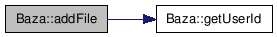
\includegraphics[width=122pt]{a00001_abbda65be49dfb28b1a578d0383599fa_cgraph}
\end{center}
\end{figure}
\hypertarget{a00001_bef61cc396e46d347a47c75e9ef8dfde}{
\index{Baza@{Baza}!connect@{connect}}
\index{connect@{connect}!Baza@{Baza}}
\subsubsection[{connect}]{\setlength{\rightskip}{0pt plus 5cm}void Baza::connect (const char $\ast$ {\em server}, \/  const char $\ast$ {\em login}, \/  const char $\ast$ {\em pass}, \/  const char $\ast$ {\em db})}}
\label{a00001_bef61cc396e46d347a47c75e9ef8dfde}


Łaczy się z bazą damych. 



I zamykamy połączenie 

Definicja w linii 3 pliku baza.cpp.

Here is the caller graph for this function:\nopagebreak
\begin{figure}[H]
\begin{center}
\leavevmode
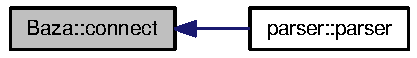
\includegraphics[width=118pt]{a00001_bef61cc396e46d347a47c75e9ef8dfde_icgraph}
\end{center}
\end{figure}
\hypertarget{a00001_a09b37e4665bd7b2f2b8b54f8120f5be}{
\index{Baza@{Baza}!get\_\-passwd@{get\_\-passwd}}
\index{get\_\-passwd@{get\_\-passwd}!Baza@{Baza}}
\subsubsection[{get\_\-passwd}]{\setlength{\rightskip}{0pt plus 5cm}std::string Baza::get\_\-passwd (std::string {\em login})}}
\label{a00001_a09b37e4665bd7b2f2b8b54f8120f5be}


Pobiera hasło uzytkownika z bazy. 



Definicja w linii 30 pliku baza.cpp.\hypertarget{a00001_1d1cfca062ab3117b2b97281df012823}{
\index{Baza@{Baza}!getFileInfo@{getFileInfo}}
\index{getFileInfo@{getFileInfo}!Baza@{Baza}}
\subsubsection[{getFileInfo}]{\setlength{\rightskip}{0pt plus 5cm}mysqlpp::StoreQueryResult Baza::getFileInfo (std::string {\em file}, \/  int {\em user\_\-id})}}
\label{a00001_1d1cfca062ab3117b2b97281df012823}




Definicja w linii 201 pliku baza.cpp.\hypertarget{a00001_e4a033a65cb585aa91c15fd8b8fde764}{
\index{Baza@{Baza}!getFileInfo@{getFileInfo}}
\index{getFileInfo@{getFileInfo}!Baza@{Baza}}
\subsubsection[{getFileInfo}]{\setlength{\rightskip}{0pt plus 5cm}mysqlpp::StoreQueryResult Baza::getFileInfo (std::string {\em file}, \/  std::string {\em user})}}
\label{a00001_e4a033a65cb585aa91c15fd8b8fde764}


Podobnie jak getFilesList tylko ze pobiera informację o jednym pliku. 



Definicja w linii 174 pliku baza.cpp.

Oto graf wywołań dla tej funkcji:\nopagebreak
\begin{figure}[H]
\begin{center}
\leavevmode
\includegraphics[width=129pt]{a00001_e4a033a65cb585aa91c15fd8b8fde764_cgraph}
\end{center}
\end{figure}
\hypertarget{a00001_2eace36725672b3a4ce639f91fe7d9bd}{
\index{Baza@{Baza}!getFilesList@{getFilesList}}
\index{getFilesList@{getFilesList}!Baza@{Baza}}
\subsubsection[{getFilesList}]{\setlength{\rightskip}{0pt plus 5cm}mysqlpp::StoreQueryResult Baza::getFilesList (std::string {\em user})}}
\label{a00001_2eace36725672b3a4ce639f91fe7d9bd}


Najpierw wywołuje \hyperlink{a00001_65054f08c8fd7c600f6c2fe2c7f61a43}{getUserId()} potem z id otrzymanym z tamtąd wywołuje \hyperlink{a00001_02db3388d088212bd443ee39998b5cf8}{getFilesList(int user\_\-id)};. 

Zapytanie o listę plików uzytkownika o nazwie podanej w zmiennej user. 

Definicja w linii 97 pliku baza.cpp.

Oto graf wywołań dla tej funkcji:\nopagebreak
\begin{figure}[H]
\begin{center}
\leavevmode
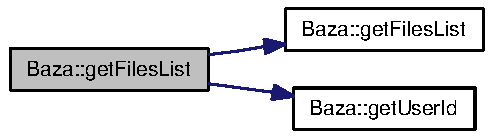
\includegraphics[width=136pt]{a00001_2eace36725672b3a4ce639f91fe7d9bd_cgraph}
\end{center}
\end{figure}
\hypertarget{a00001_02db3388d088212bd443ee39998b5cf8}{
\index{Baza@{Baza}!getFilesList@{getFilesList}}
\index{getFilesList@{getFilesList}!Baza@{Baza}}
\subsubsection[{getFilesList}]{\setlength{\rightskip}{0pt plus 5cm}mysqlpp::StoreQueryResult Baza::getFilesList (int {\em user\_\-id})}}
\label{a00001_02db3388d088212bd443ee39998b5cf8}


Pobiera listę plików z bazy na podstawie ID uzytkownika. 

Zapytanie o listę plikow uzytkownika po id uzytkownika z bazy accounts\_\-konto. 

Definicja w linii 61 pliku baza.cpp.

Here is the caller graph for this function:\nopagebreak
\begin{figure}[H]
\begin{center}
\leavevmode
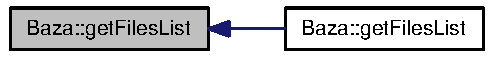
\includegraphics[width=136pt]{a00001_02db3388d088212bd443ee39998b5cf8_icgraph}
\end{center}
\end{figure}
\hypertarget{a00001_65054f08c8fd7c600f6c2fe2c7f61a43}{
\index{Baza@{Baza}!getUserId@{getUserId}}
\index{getUserId@{getUserId}!Baza@{Baza}}
\subsubsection[{getUserId}]{\setlength{\rightskip}{0pt plus 5cm}int Baza::getUserId (std::string {\em user})}}
\label{a00001_65054f08c8fd7c600f6c2fe2c7f61a43}


Pobiera id uzytkownika 'user'. 

Zapytanie o ID uzytkownika o loginie 'user' ale nie o id z auth\_\-user tylko o id z accounts\_\-konto. 

Definicja w linii 126 pliku baza.cpp.

Here is the caller graph for this function:\nopagebreak
\begin{figure}[H]
\begin{center}
\leavevmode
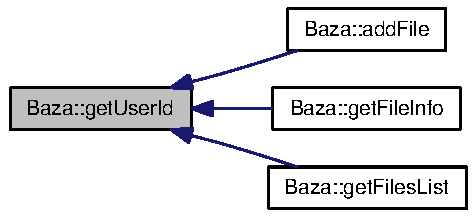
\includegraphics[width=132pt]{a00001_65054f08c8fd7c600f6c2fe2c7f61a43_icgraph}
\end{center}
\end{figure}
\hypertarget{a00001_7161c573401166cc5f7d98ae6f335b44}{
\index{Baza@{Baza}!rmFile@{rmFile}}
\index{rmFile@{rmFile}!Baza@{Baza}}
\subsubsection[{rmFile}]{\setlength{\rightskip}{0pt plus 5cm}bool Baza::rmFile (std::string {\em nazwa}, \/  std::string {\em konto}, \/  std::string {\em hash})}}
\label{a00001_7161c573401166cc5f7d98ae6f335b44}


Usuwa plik z bazy \begin{Desc}
\item[Parametry:]
\begin{description}
\item[{\em nazwa}]nazwa pliku do usuniecia \item[{\em konto}]nazwa konta z ktorego sie usuwa \item[{\em hash}]hash pliku (dla sprawdzenia czy napewno dobry plik) \end{description}
\end{Desc}
\begin{Desc}
\item[Zwraca:]czy operacja zakończona powodzeniem \end{Desc}


Dokumentacja dla tej klasy została wygenerowana z plików:\begin{CompactItemize}
\item 
/home/pawel/Dokumenty/Uczelnia/grupappz/Source/Ass8-server/\hyperlink{a00007}{baza.hpp}\item 
/home/pawel/Dokumenty/Uczelnia/grupappz/Source/Ass8-server/\hyperlink{a00006}{baza.cpp}\end{CompactItemize}

\hypertarget{a00002}{
\section{Dokumentacja klasy MD5}
\label{d7/d46/a00002}\index{MD5@{MD5}}
}
{\tt \#include $<$md5.h$>$}

\subsection*{Metody publiczne}
\begin{CompactItemize}
\item 
void \hyperlink{a00002_72b35c041cb6983aaa74e2f1c31d5a29}{MD5Init} (\hyperlink{a00003}{MD5\_\-CTX} $\ast$)
\item 
void \hyperlink{a00002_a59116f0a26354a217fa186a43cd9d28}{MD5Update} (\hyperlink{a00003}{MD5\_\-CTX} $\ast$, unsigned char $\ast$, unsigned int)
\item 
void \hyperlink{a00002_98039031d87c1f5b787050e2b487d83f}{MD5Final} (unsigned char\mbox{[}16\mbox{]}, \hyperlink{a00003}{MD5\_\-CTX} $\ast$)
\item 
\hyperlink{a00002_fa6155ec36de415ab2dcf5e54b670d13}{MD5} ()
\end{CompactItemize}
\subsection*{Metody prywatne}
\begin{CompactItemize}
\item 
void \hyperlink{a00002_849ad3347bad15a23f3a40452476b1e0}{MD5Transform} (unsigned long int state\mbox{[}4\mbox{]}, unsigned char block\mbox{[}64\mbox{]})
\item 
void \hyperlink{a00002_c3c05716498203127920ba78b3ae8115}{Encode} (unsigned char $\ast$, unsigned long int $\ast$, unsigned int)
\item 
void \hyperlink{a00002_ef62580b93f2122c62493464787b814a}{Decode} (unsigned long int $\ast$, unsigned char $\ast$, unsigned int)
\item 
void \hyperlink{a00002_76c181f092e81df65dadf8861272ac80}{MD5\_\-memcpy} (\hyperlink{a00011_73204e40637f83518fb695362ea084a4}{POINTER}, \hyperlink{a00011_73204e40637f83518fb695362ea084a4}{POINTER}, unsigned int)
\item 
void \hyperlink{a00002_e1a522aab83da49d1bd3f0a6f3edcd11}{MD5\_\-memset} (\hyperlink{a00011_73204e40637f83518fb695362ea084a4}{POINTER}, int, unsigned int)
\end{CompactItemize}


\subsection{Opis szczegółowy}


Definicja w linii 60 pliku md5.h.

\subsection{Dokumentacja konstruktora i destruktora}
\hypertarget{a00002_fa6155ec36de415ab2dcf5e54b670d13}{
\index{MD5@{MD5}!MD5@{MD5}}
\index{MD5@{MD5}!MD5@{MD5}}
\subsubsection[{MD5}]{\setlength{\rightskip}{0pt plus 5cm}MD5::MD5 ()\hspace{0.3cm}{\tt  \mbox{[}inline\mbox{]}}}}
\label{d7/d46/a00002_fa6155ec36de415ab2dcf5e54b670d13}




Definicja w linii 77 pliku md5.h.

\subsection{Dokumentacja funkcji składowych}
\hypertarget{a00002_ef62580b93f2122c62493464787b814a}{
\index{MD5@{MD5}!Decode@{Decode}}
\index{Decode@{Decode}!MD5@{MD5}}
\subsubsection[{Decode}]{\setlength{\rightskip}{0pt plus 5cm}void MD5::Decode (unsigned long int $\ast$ {\em output}, \/  unsigned char $\ast$ {\em input}, \/  unsigned int {\em len})\hspace{0.3cm}{\tt  \mbox{[}private\mbox{]}}}}
\label{d7/d46/a00002_ef62580b93f2122c62493464787b814a}




Definicja w linii 293 pliku md5.cpp.

Here is the caller graph for this function:\nopagebreak
\begin{figure}[H]
\begin{center}
\leavevmode
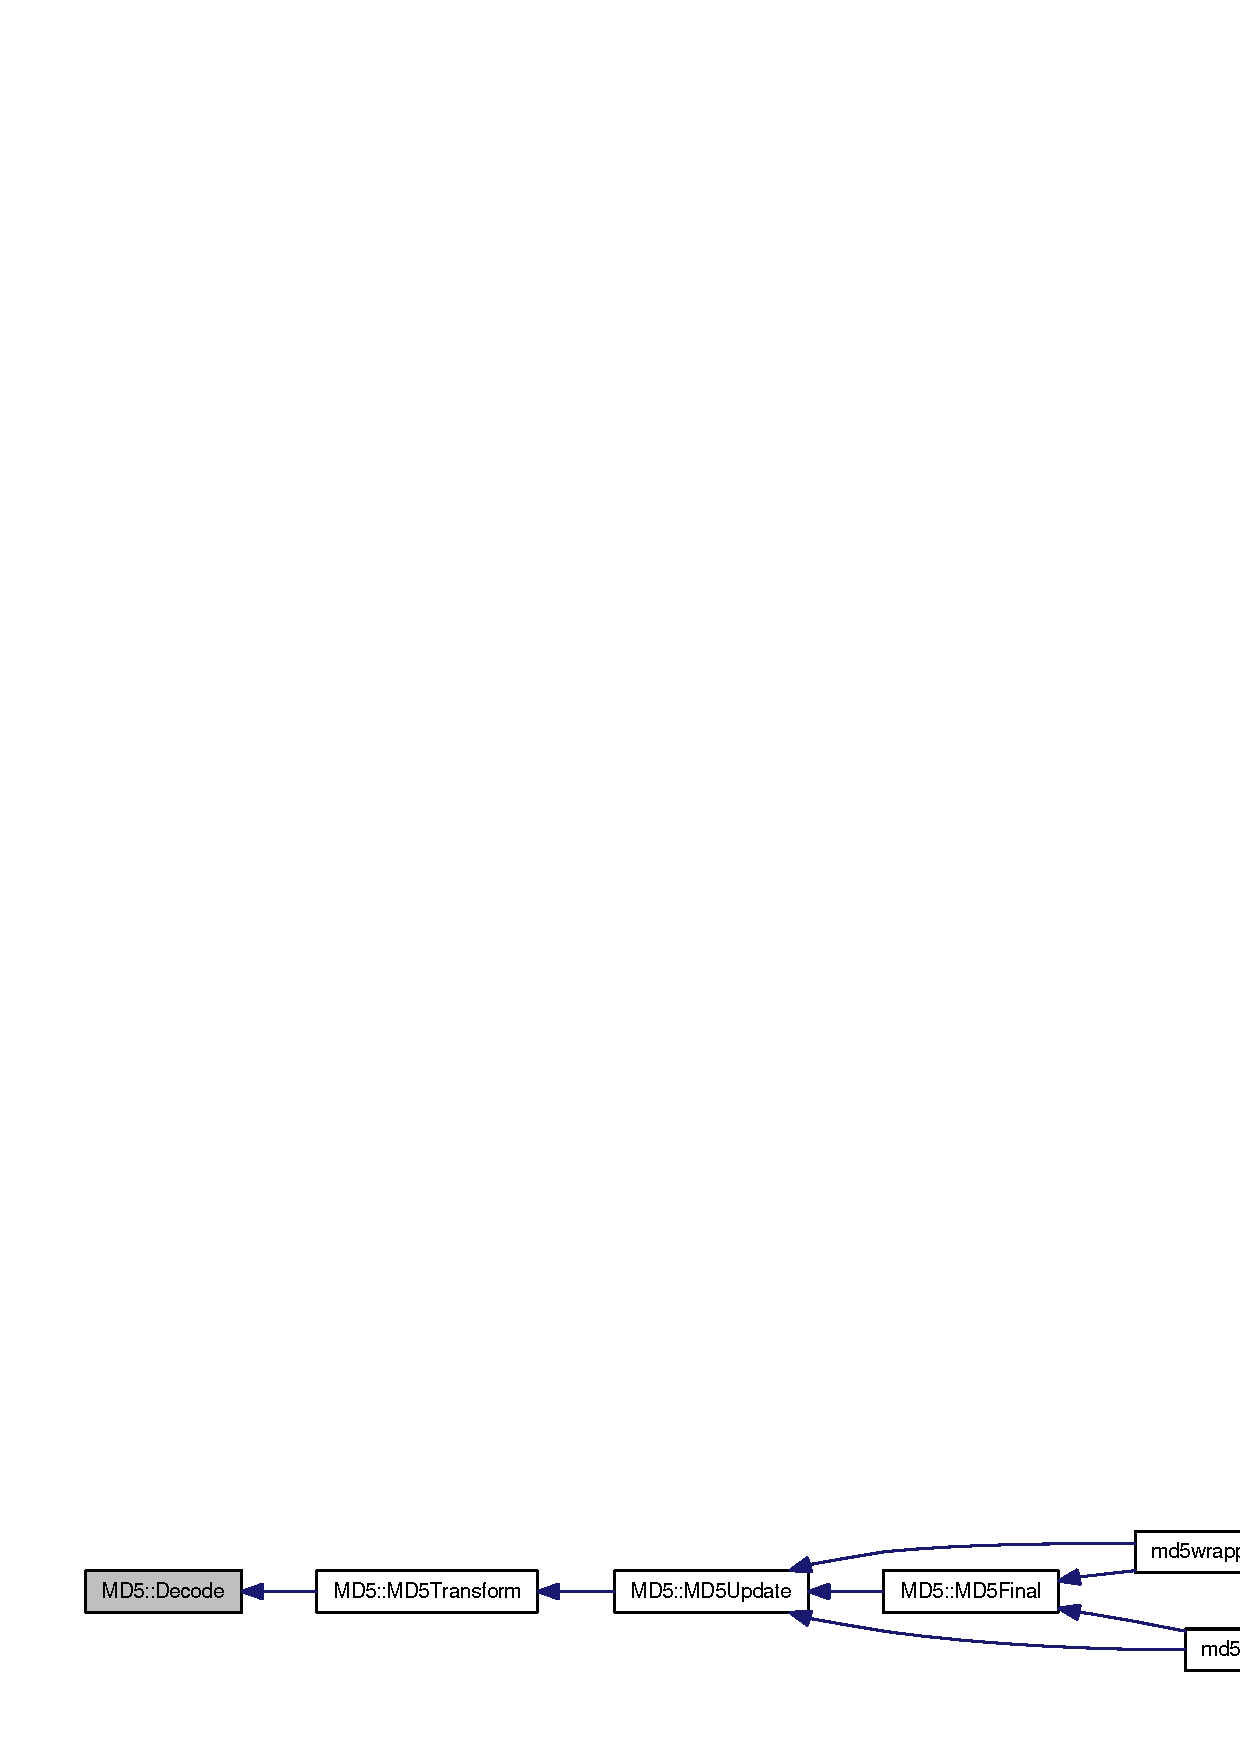
\includegraphics[width=420pt]{d7/d46/a00002_ef62580b93f2122c62493464787b814a_icgraph}
\end{center}
\end{figure}
\hypertarget{a00002_c3c05716498203127920ba78b3ae8115}{
\index{MD5@{MD5}!Encode@{Encode}}
\index{Encode@{Encode}!MD5@{MD5}}
\subsubsection[{Encode}]{\setlength{\rightskip}{0pt plus 5cm}void MD5::Encode (unsigned char $\ast$ {\em output}, \/  unsigned long int $\ast$ {\em input}, \/  unsigned int {\em len})\hspace{0.3cm}{\tt  \mbox{[}private\mbox{]}}}}
\label{d7/d46/a00002_c3c05716498203127920ba78b3ae8115}




Definicja w linii 277 pliku md5.cpp.

Here is the caller graph for this function:\nopagebreak
\begin{figure}[H]
\begin{center}
\leavevmode
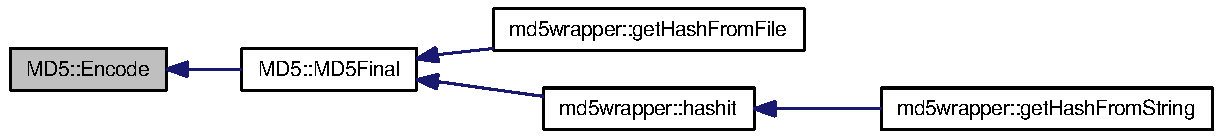
\includegraphics[width=311pt]{d7/d46/a00002_c3c05716498203127920ba78b3ae8115_icgraph}
\end{center}
\end{figure}
\hypertarget{a00002_76c181f092e81df65dadf8861272ac80}{
\index{MD5@{MD5}!MD5\_\-memcpy@{MD5\_\-memcpy}}
\index{MD5\_\-memcpy@{MD5\_\-memcpy}!MD5@{MD5}}
\subsubsection[{MD5\_\-memcpy}]{\setlength{\rightskip}{0pt plus 5cm}void MD5::MD5\_\-memcpy ({\bf POINTER} {\em output}, \/  {\bf POINTER} {\em input}, \/  unsigned int {\em len})\hspace{0.3cm}{\tt  \mbox{[}private\mbox{]}}}}
\label{d7/d46/a00002_76c181f092e81df65dadf8861272ac80}




Definicja w linii 307 pliku md5.cpp.

Here is the caller graph for this function:\nopagebreak
\begin{figure}[H]
\begin{center}
\leavevmode
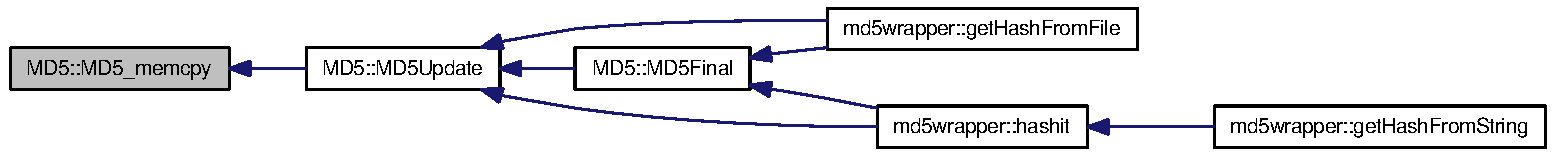
\includegraphics[width=391pt]{d7/d46/a00002_76c181f092e81df65dadf8861272ac80_icgraph}
\end{center}
\end{figure}
\hypertarget{a00002_e1a522aab83da49d1bd3f0a6f3edcd11}{
\index{MD5@{MD5}!MD5\_\-memset@{MD5\_\-memset}}
\index{MD5\_\-memset@{MD5\_\-memset}!MD5@{MD5}}
\subsubsection[{MD5\_\-memset}]{\setlength{\rightskip}{0pt plus 5cm}void MD5::MD5\_\-memset ({\bf POINTER} {\em output}, \/  int {\em value}, \/  unsigned int {\em len})\hspace{0.3cm}{\tt  \mbox{[}private\mbox{]}}}}
\label{d7/d46/a00002_e1a522aab83da49d1bd3f0a6f3edcd11}




Definicja w linii 318 pliku md5.cpp.

Here is the caller graph for this function:\nopagebreak
\begin{figure}[H]
\begin{center}
\leavevmode
\includegraphics[width=420pt]{d7/d46/a00002_e1a522aab83da49d1bd3f0a6f3edcd11_icgraph}
\end{center}
\end{figure}
\hypertarget{a00002_98039031d87c1f5b787050e2b487d83f}{
\index{MD5@{MD5}!MD5Final@{MD5Final}}
\index{MD5Final@{MD5Final}!MD5@{MD5}}
\subsubsection[{MD5Final}]{\setlength{\rightskip}{0pt plus 5cm}void MD5::MD5Final (unsigned char {\em digest}\mbox{[}16\mbox{]}, \/  {\bf MD5\_\-CTX} $\ast$ {\em context})}}
\label{d7/d46/a00002_98039031d87c1f5b787050e2b487d83f}




Definicja w linii 153 pliku md5.cpp.

Oto graf wywołań dla tej funkcji:\nopagebreak
\begin{figure}[H]
\begin{center}
\leavevmode
\includegraphics[width=270pt]{d7/d46/a00002_98039031d87c1f5b787050e2b487d83f_cgraph}
\end{center}
\end{figure}


Here is the caller graph for this function:\nopagebreak
\begin{figure}[H]
\begin{center}
\leavevmode
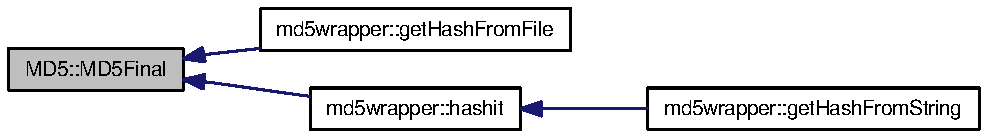
\includegraphics[width=255pt]{d7/d46/a00002_98039031d87c1f5b787050e2b487d83f_icgraph}
\end{center}
\end{figure}
\hypertarget{a00002_72b35c041cb6983aaa74e2f1c31d5a29}{
\index{MD5@{MD5}!MD5Init@{MD5Init}}
\index{MD5Init@{MD5Init}!MD5@{MD5}}
\subsubsection[{MD5Init}]{\setlength{\rightskip}{0pt plus 5cm}void MD5::MD5Init ({\bf MD5\_\-CTX} $\ast$ {\em context})}}
\label{d7/d46/a00002_72b35c041cb6983aaa74e2f1c31d5a29}




Definicja w linii 98 pliku md5.cpp.

Here is the caller graph for this function:\nopagebreak
\begin{figure}[H]
\begin{center}
\leavevmode
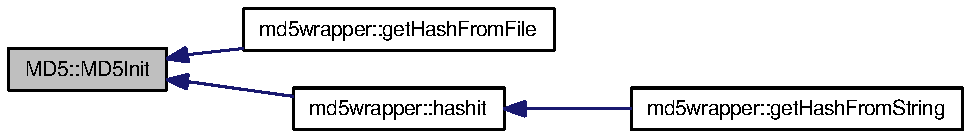
\includegraphics[width=251pt]{d7/d46/a00002_72b35c041cb6983aaa74e2f1c31d5a29_icgraph}
\end{center}
\end{figure}
\hypertarget{a00002_849ad3347bad15a23f3a40452476b1e0}{
\index{MD5@{MD5}!MD5Transform@{MD5Transform}}
\index{MD5Transform@{MD5Transform}!MD5@{MD5}}
\subsubsection[{MD5Transform}]{\setlength{\rightskip}{0pt plus 5cm}void MD5::MD5Transform (unsigned long int {\em state}\mbox{[}4\mbox{]}, \/  unsigned char {\em block}\mbox{[}64\mbox{]})\hspace{0.3cm}{\tt  \mbox{[}private\mbox{]}}}}
\label{d7/d46/a00002_849ad3347bad15a23f3a40452476b1e0}




Definicja w linii 183 pliku md5.cpp.

Oto graf wywołań dla tej funkcji:\nopagebreak
\begin{figure}[H]
\begin{center}
\leavevmode
\includegraphics[width=145pt]{d7/d46/a00002_849ad3347bad15a23f3a40452476b1e0_cgraph}
\end{center}
\end{figure}


Here is the caller graph for this function:\nopagebreak
\begin{figure}[H]
\begin{center}
\leavevmode
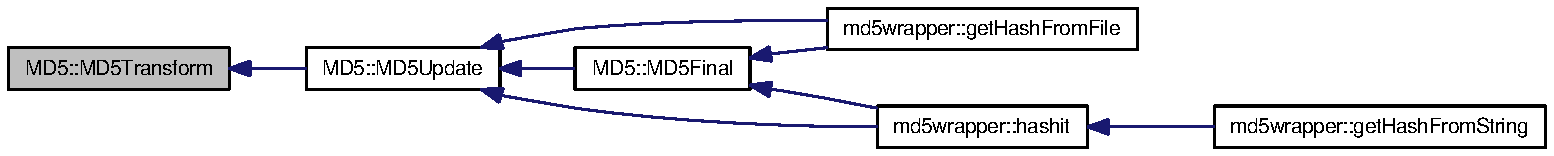
\includegraphics[width=391pt]{d7/d46/a00002_849ad3347bad15a23f3a40452476b1e0_icgraph}
\end{center}
\end{figure}
\hypertarget{a00002_a59116f0a26354a217fa186a43cd9d28}{
\index{MD5@{MD5}!MD5Update@{MD5Update}}
\index{MD5Update@{MD5Update}!MD5@{MD5}}
\subsubsection[{MD5Update}]{\setlength{\rightskip}{0pt plus 5cm}void MD5::MD5Update ({\bf MD5\_\-CTX} $\ast$ {\em context}, \/  unsigned char $\ast$ {\em input}, \/  unsigned int {\em inputLen})}}
\label{d7/d46/a00002_a59116f0a26354a217fa186a43cd9d28}




Definicja w linii 112 pliku md5.cpp.

Oto graf wywołań dla tej funkcji:\nopagebreak
\begin{figure}[H]
\begin{center}
\leavevmode
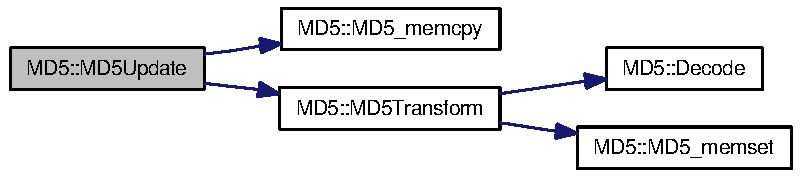
\includegraphics[width=210pt]{d7/d46/a00002_a59116f0a26354a217fa186a43cd9d28_cgraph}
\end{center}
\end{figure}


Here is the caller graph for this function:\nopagebreak
\begin{figure}[H]
\begin{center}
\leavevmode
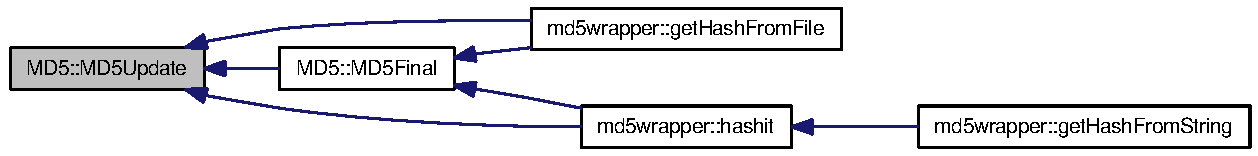
\includegraphics[width=320pt]{d7/d46/a00002_a59116f0a26354a217fa186a43cd9d28_icgraph}
\end{center}
\end{figure}


Dokumentacja dla tej klasy została wygenerowana z plików:\begin{CompactItemize}
\item 
\hyperlink{a00011}{md5.h}\item 
\hyperlink{a00010}{md5.cpp}\end{CompactItemize}

\chapter{Dokumentacja plików}
\hypertarget{a00003}{
\section{Dokumentacja struktury MD5\_\-CTX}
\label{d1/d7c/a00003}\index{MD5\_\-CTX@{MD5\_\-CTX}}
}
{\tt \#include $<$md5.h$>$}

\subsection*{Atrybuty publiczne}
\begin{CompactItemize}
\item 
unsigned long int \hyperlink{a00003_2f697997f51de65d08227fdf1d5c44b8}{state} \mbox{[}4\mbox{]}
\item 
unsigned long int \hyperlink{a00003_889cb6e121b82a1e7f4d92120fb8a523}{count} \mbox{[}2\mbox{]}
\item 
unsigned char \hyperlink{a00003_2da73ecf544745f58211e998719f367f}{buffer} \mbox{[}64\mbox{]}
\end{CompactItemize}


\subsection{Opis szczegółowy}


Definicja w linii 50 pliku md5.h.

\subsection{Dokumentacja atrybutów składowych}
\hypertarget{a00003_2da73ecf544745f58211e998719f367f}{
\index{MD5\_\-CTX@{MD5\_\-CTX}!buffer@{buffer}}
\index{buffer@{buffer}!MD5_CTX@{MD5\_\-CTX}}
\subsubsection[{buffer}]{\setlength{\rightskip}{0pt plus 5cm}unsigned char {\bf MD5\_\-CTX::buffer}\mbox{[}64\mbox{]}}}
\label{d1/d7c/a00003_2da73ecf544745f58211e998719f367f}




Definicja w linii 54 pliku md5.h.\hypertarget{a00003_889cb6e121b82a1e7f4d92120fb8a523}{
\index{MD5\_\-CTX@{MD5\_\-CTX}!count@{count}}
\index{count@{count}!MD5_CTX@{MD5\_\-CTX}}
\subsubsection[{count}]{\setlength{\rightskip}{0pt plus 5cm}unsigned long int {\bf MD5\_\-CTX::count}\mbox{[}2\mbox{]}}}
\label{d1/d7c/a00003_889cb6e121b82a1e7f4d92120fb8a523}




Definicja w linii 53 pliku md5.h.\hypertarget{a00003_2f697997f51de65d08227fdf1d5c44b8}{
\index{MD5\_\-CTX@{MD5\_\-CTX}!state@{state}}
\index{state@{state}!MD5_CTX@{MD5\_\-CTX}}
\subsubsection[{state}]{\setlength{\rightskip}{0pt plus 5cm}unsigned long int {\bf MD5\_\-CTX::state}\mbox{[}4\mbox{]}}}
\label{d1/d7c/a00003_2f697997f51de65d08227fdf1d5c44b8}




Definicja w linii 52 pliku md5.h.

Dokumentacja dla tej struktury została wygenerowana z pliku:\begin{CompactItemize}
\item 
\hyperlink{a00011}{md5.h}\end{CompactItemize}

\hypertarget{a00004}{
\section{Dokumentacja klasy md5wrapper}
\label{d0/d0b/a00004}\index{md5wrapper@{md5wrapper}}
}
{\tt \#include $<$md5wrapper.h$>$}

Diagram współpracy dla md5wrapper:\nopagebreak
\begin{figure}[H]
\begin{center}
\leavevmode
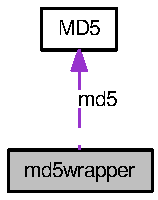
\includegraphics[width=112pt]{d4/d6d/a00055}
\end{center}
\end{figure}
\subsection*{Metody publiczne}
\begin{CompactItemize}
\item 
\hyperlink{a00004_ae8138b76b89d93a4c21077b76d57c07}{md5wrapper} ()
\item 
\hyperlink{a00004_65e78258ad508d83be81d395f8bd43f4}{$\sim$md5wrapper} ()
\item 
std::string \hyperlink{a00004_225ba5a78228b867c3f17fdba959d8e6}{getHashFromString} (std::string text)
\item 
std::string \hyperlink{a00004_e6cd2a7928b997c5d6388ae81a0d841a}{getHashFromFile} (std::string filename)
\end{CompactItemize}
\subsection*{Metody prywatne}
\begin{CompactItemize}
\item 
std::string \hyperlink{a00004_608ecf61c0ecdf2fcb772e9fd6c51d5f}{hashit} (std::string text)
\item 
std::string \hyperlink{a00004_74f856c53740d3beb133074baffd21aa}{convToString} (unsigned char $\ast$bytes)
\end{CompactItemize}
\subsection*{Atrybuty prywatne}
\begin{CompactItemize}
\item 
\hyperlink{a00002}{MD5} $\ast$ \hyperlink{a00004_fe675f7d8993ec64ddefa902dff431fa}{md5}
\end{CompactItemize}


\subsection{Opis szczegółowy}


Definicja w linii 23 pliku md5wrapper.h.

\subsection{Dokumentacja konstruktora i destruktora}
\hypertarget{a00004_ae8138b76b89d93a4c21077b76d57c07}{
\index{md5wrapper@{md5wrapper}!md5wrapper@{md5wrapper}}
\index{md5wrapper@{md5wrapper}!md5wrapper@{md5wrapper}}
\subsubsection[{md5wrapper}]{\setlength{\rightskip}{0pt plus 5cm}md5wrapper::md5wrapper ()}}
\label{d0/d0b/a00004_ae8138b76b89d93a4c21077b76d57c07}




Definicja w linii 70 pliku md5wrapper.cpp.\hypertarget{a00004_65e78258ad508d83be81d395f8bd43f4}{
\index{md5wrapper@{md5wrapper}!$\sim$md5wrapper@{$\sim$md5wrapper}}
\index{$\sim$md5wrapper@{$\sim$md5wrapper}!md5wrapper@{md5wrapper}}
\subsubsection[{$\sim$md5wrapper}]{\setlength{\rightskip}{0pt plus 5cm}md5wrapper::$\sim$md5wrapper ()}}
\label{d0/d0b/a00004_65e78258ad508d83be81d395f8bd43f4}




Definicja w linii 77 pliku md5wrapper.cpp.

\subsection{Dokumentacja funkcji składowych}
\hypertarget{a00004_74f856c53740d3beb133074baffd21aa}{
\index{md5wrapper@{md5wrapper}!convToString@{convToString}}
\index{convToString@{convToString}!md5wrapper@{md5wrapper}}
\subsubsection[{convToString}]{\setlength{\rightskip}{0pt plus 5cm}std::string md5wrapper::convToString (unsigned char $\ast$ {\em bytes})\hspace{0.3cm}{\tt  \mbox{[}private\mbox{]}}}}
\label{d0/d0b/a00004_74f856c53740d3beb133074baffd21aa}




Definicja w linii 53 pliku md5wrapper.cpp.

Here is the caller graph for this function:\nopagebreak
\begin{figure}[H]
\begin{center}
\leavevmode
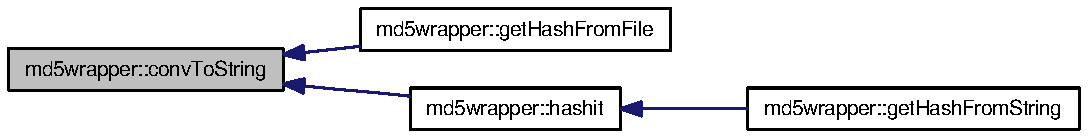
\includegraphics[width=279pt]{d0/d0b/a00004_74f856c53740d3beb133074baffd21aa_icgraph}
\end{center}
\end{figure}
\hypertarget{a00004_e6cd2a7928b997c5d6388ae81a0d841a}{
\index{md5wrapper@{md5wrapper}!getHashFromFile@{getHashFromFile}}
\index{getHashFromFile@{getHashFromFile}!md5wrapper@{md5wrapper}}
\subsubsection[{getHashFromFile}]{\setlength{\rightskip}{0pt plus 5cm}std::string md5wrapper::getHashFromFile (std::string {\em filename})}}
\label{d0/d0b/a00004_e6cd2a7928b997c5d6388ae81a0d841a}




Definicja w linii 100 pliku md5wrapper.cpp.

Oto graf wywołań dla tej funkcji:\nopagebreak
\begin{figure}[H]
\begin{center}
\leavevmode
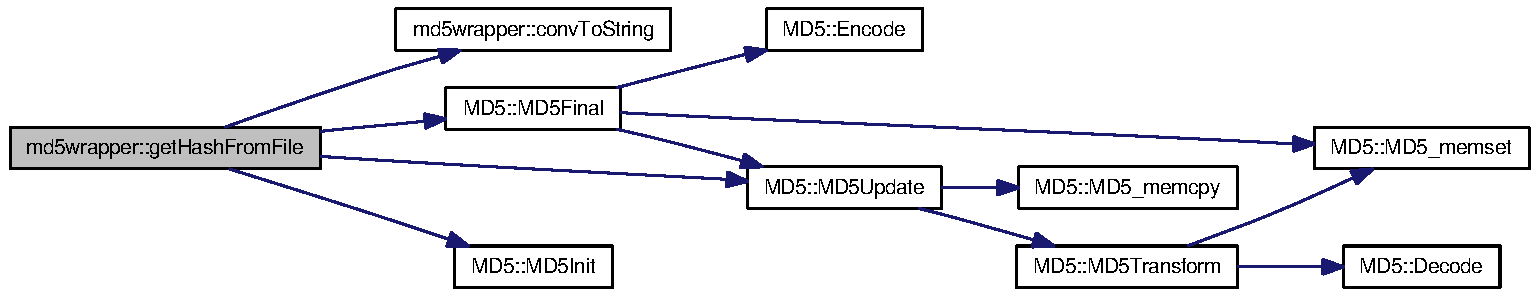
\includegraphics[width=387pt]{d0/d0b/a00004_e6cd2a7928b997c5d6388ae81a0d841a_cgraph}
\end{center}
\end{figure}
\hypertarget{a00004_225ba5a78228b867c3f17fdba959d8e6}{
\index{md5wrapper@{md5wrapper}!getHashFromString@{getHashFromString}}
\index{getHashFromString@{getHashFromString}!md5wrapper@{md5wrapper}}
\subsubsection[{getHashFromString}]{\setlength{\rightskip}{0pt plus 5cm}std::string md5wrapper::getHashFromString (std::string {\em text})}}
\label{d0/d0b/a00004_225ba5a78228b867c3f17fdba959d8e6}




Definicja w linii 87 pliku md5wrapper.cpp.

Oto graf wywołań dla tej funkcji:\nopagebreak
\begin{figure}[H]
\begin{center}
\leavevmode
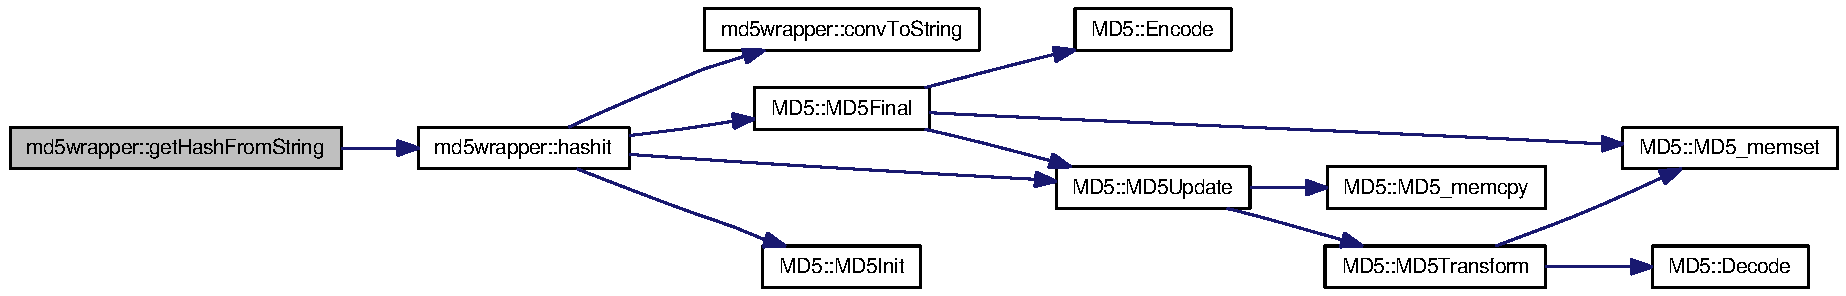
\includegraphics[width=420pt]{d0/d0b/a00004_225ba5a78228b867c3f17fdba959d8e6_cgraph}
\end{center}
\end{figure}
\hypertarget{a00004_608ecf61c0ecdf2fcb772e9fd6c51d5f}{
\index{md5wrapper@{md5wrapper}!hashit@{hashit}}
\index{hashit@{hashit}!md5wrapper@{md5wrapper}}
\subsubsection[{hashit}]{\setlength{\rightskip}{0pt plus 5cm}std::string md5wrapper::hashit (std::string {\em text})\hspace{0.3cm}{\tt  \mbox{[}private\mbox{]}}}}
\label{d0/d0b/a00004_608ecf61c0ecdf2fcb772e9fd6c51d5f}




Definicja w linii 28 pliku md5wrapper.cpp.

Oto graf wywołań dla tej funkcji:\nopagebreak
\begin{figure}[H]
\begin{center}
\leavevmode
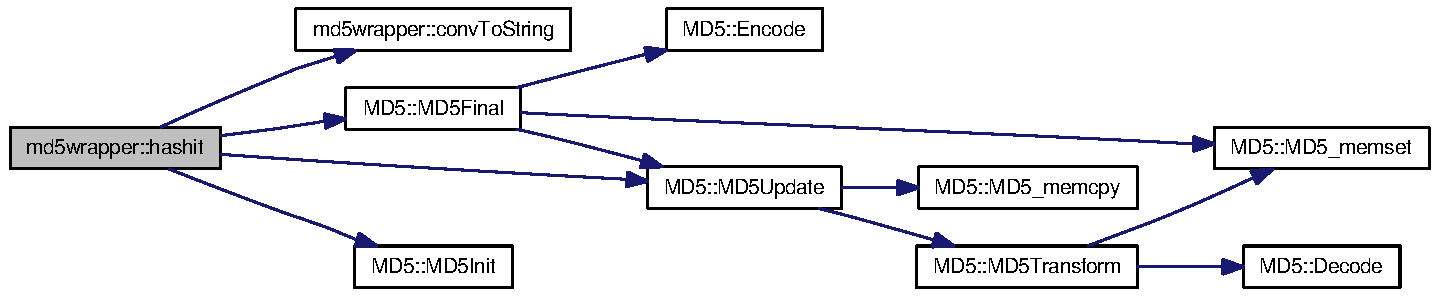
\includegraphics[width=363pt]{d0/d0b/a00004_608ecf61c0ecdf2fcb772e9fd6c51d5f_cgraph}
\end{center}
\end{figure}


Here is the caller graph for this function:\nopagebreak
\begin{figure}[H]
\begin{center}
\leavevmode
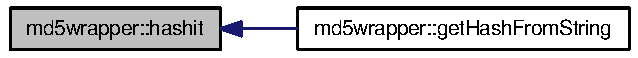
\includegraphics[width=171pt]{d0/d0b/a00004_608ecf61c0ecdf2fcb772e9fd6c51d5f_icgraph}
\end{center}
\end{figure}


\subsection{Dokumentacja atrybutów składowych}
\hypertarget{a00004_fe675f7d8993ec64ddefa902dff431fa}{
\index{md5wrapper@{md5wrapper}!md5@{md5}}
\index{md5@{md5}!md5wrapper@{md5wrapper}}
\subsubsection[{md5}]{\setlength{\rightskip}{0pt plus 5cm}{\bf MD5}$\ast$ {\bf md5wrapper::md5}\hspace{0.3cm}{\tt  \mbox{[}private\mbox{]}}}}
\label{d0/d0b/a00004_fe675f7d8993ec64ddefa902dff431fa}




Definicja w linii 26 pliku md5wrapper.h.

Dokumentacja dla tej klasy została wygenerowana z plików:\begin{CompactItemize}
\item 
/home/pawel/Dokumenty/Uczelnia/grupappz/Source/Ass8-server/include/md5/\hyperlink{a00012}{md5wrapper.h}\item 
/home/pawel/Dokumenty/Uczelnia/grupappz/Source/Ass8-server/include/md5/\hyperlink{a00011}{md5wrapper.cpp}\end{CompactItemize}

\hypertarget{a00005}{
\section{Dokumentacja klasy parser}
\label{dd/dad/a00005}\index{parser@{parser}}
}
{\tt \#include $<$parser.hpp$>$}

Diagram współpracy dla parser:\nopagebreak
\begin{figure}[H]
\begin{center}
\leavevmode
\includegraphics[width=189pt]{d9/d73/a00060}
\end{center}
\end{figure}
\subsection*{Metody publiczne}
\begin{CompactItemize}
\item 
\hyperlink{a00005_3a237071a3ab764cd61bc53df9dd4f46}{parser} (tcp::iostream \&\hyperlink{a00005_f95fb0cac229181329fa61f7bc72c65b}{stream}, const char $\ast$server, const char $\ast$user, const char $\ast$pass, const char $\ast$db)
\item 
void \hyperlink{a00005_7793913f528921aa22c4b6cc259a0a14}{start} ()
\end{CompactItemize}
\subsection*{Metody prywatne}
\begin{CompactItemize}
\item 
bool \hyperlink{a00005_9ce7290217bd14e4efcbe2cad32ccf95}{parsuj} (std::string \&do\_\-parsowania)
\begin{CompactList}\small\item\em Parsuje dane pobrane od klienta. \item\end{CompactList}\item 
bool \hyperlink{a00005_71abf468eb72a833dbd6c8a895b66b52}{logowanie} (std::string \hyperlink{a00005_8bb124a2f285074773d1b0ee62cf0cc0}{login}, std::string \hyperlink{a00005_2fc04d16e2ba688c5b306a2ad6770039}{haslo})
\begin{CompactList}\small\item\em Loguje klienta po przetworzeniu xmla odebranego od niego i sparsownaiu go w void \hyperlink{a00005_9ce7290217bd14e4efcbe2cad32ccf95}{parsuj()}. \item\end{CompactList}\item 
void \hyperlink{a00005_6a29174f787861caadc6c2e34b99f8c0}{odpowiedz\_\-login} (int i)
\item 
void \hyperlink{a00005_49d270636d2f3d5376c3cba62b5ea839}{Odpowiedz} (int nr\_\-odpowiedzi, int numer\_\-operacji=-1)
\item 
void \hyperlink{a00005_e45404aec82f8c70a023bdc365c74287}{Odpowiedz} (int nr\_\-odpowiedzi, int nr\_\-operacji, std::string odp)
\begin{CompactList}\small\item\em Wysyła odpowiedź wielolinijkową zależnie od podanego i gdzie i jak w void \hyperlink{a00005_49d270636d2f3d5376c3cba62b5ea839}{Odpowiedz(int i, int numer\_\-operacji)};. \item\end{CompactList}\item 
void \hyperlink{a00005_2f6aceaa94a28fc699e4f824f7622b51}{wyslij} (std::string w)
\begin{CompactList}\small\item\em Wysyła dane podane w stringu w dodatkowo wysyłając znak końca linii. \item\end{CompactList}\item 
void \hyperlink{a00005_96f941201d172eeaf2fb4d8429edfc0c}{lista\_\-plikow} (std::string uzytkownik)
\begin{CompactList}\small\item\em Wysyła listę plików użytkownika 'uzytkownik'. \item\end{CompactList}\item 
void \hyperlink{a00005_4e084ae10e8498b171c44a0138597d2e}{odbieranie\_\-plikow} (xmlpp::TextReader \&reader, std::string uzytkownik)
\begin{CompactList}\small\item\em Odbiera plik od użytkownika i umieszcza na serwerze. \item\end{CompactList}\item 
void \hyperlink{a00005_cc293df6220f5030fab5a7ee9cf8b1fa}{wysylanie\_\-plikow} (xmlpp::TextReader \&reader, std::string uzytkownil)
\begin{CompactList}\small\item\em Odbiera od klienta informację jakie on chce pobrać pliki i przekazuje kazdy plik pojedynczo do \hyperlink{a00005_771537f72f9e6a9cdb1d2961828eb66b}{wyslij\_\-plik()}. \item\end{CompactList}\item 
void \hyperlink{a00005_7ef79f818429f70b9cb35c0a33b59a10}{usun\_\-pliki} (xmlpp::TextReader \&reader, std::string uzytkownik)
\begin{CompactList}\small\item\em Usuwa plik z serwera (jeszcze nie zaimplementowane). \item\end{CompactList}\item 
void \hyperlink{a00005_771537f72f9e6a9cdb1d2961828eb66b}{wyslij\_\-plik} (std::string plik, std::string uzytkownik)
\begin{CompactList}\small\item\em wysyła plik podany w argumencie \item\end{CompactList}\item 
std::vector$<$ std::string $>$ \hyperlink{a00005_05500b74ebdcc1578ead4c31fca73a5b}{pobieranie\_\-listy\_\-plikow} (xmlpp::TextReader \&reader)
\begin{CompactList}\small\item\em Przygotowuje listę plikow do wysłania do klienta. \item\end{CompactList}\item 
std::string \hyperlink{a00005_272ecc740702b4f48efdb8469b414b24}{czytanie\_\-z\_\-socketa} ()
\end{CompactItemize}
\subsection*{Atrybuty prywatne}
\begin{CompactItemize}
\item 
tcp::iostream \& \hyperlink{a00005_f95fb0cac229181329fa61f7bc72c65b}{stream}
\begin{CompactList}\small\item\em Stream uzywany do odbierania i wysyłania informacji. \item\end{CompactList}\item 
std::string \hyperlink{a00005_8bb124a2f285074773d1b0ee62cf0cc0}{login}
\begin{CompactList}\small\item\em Zmienna przechowująca login uzytkownika. \item\end{CompactList}\item 
std::string \hyperlink{a00005_2fc04d16e2ba688c5b306a2ad6770039}{haslo}
\begin{CompactList}\small\item\em Zmienna przechowująca haslo (w przyszlosci hash hasla) uzytkownika. \item\end{CompactList}\item 
int \hyperlink{a00005_aa8407d10d299b524fa2f74532e537ac}{id\_\-sesji}
\begin{CompactList}\small\item\em Aktualny ID sesji potrzebny pryz kazdym polaczneiu. \item\end{CompactList}\item 
char \hyperlink{a00005_2e7575bebca6d0fd9f5a8bfe6fc652d0}{bufor} \mbox{[}BUFSIZE\mbox{]}
\begin{CompactList}\small\item\em Bufor danych. \item\end{CompactList}\item 
\hyperlink{a00001}{Baza} \hyperlink{a00005_21b4b313249353e48f7ea67f534ee519}{baza}
\begin{CompactList}\small\item\em Clasa obsługująca bazę danych. \item\end{CompactList}\end{CompactItemize}


\subsection{Opis szczegółowy}


Definicja w linii 27 pliku parser.hpp.

\subsection{Dokumentacja konstruktora i destruktora}
\hypertarget{a00005_3a237071a3ab764cd61bc53df9dd4f46}{
\index{parser@{parser}!parser@{parser}}
\index{parser@{parser}!parser@{parser}}
\subsubsection[{parser}]{\setlength{\rightskip}{0pt plus 5cm}parser::parser (tcp::iostream \& {\em stream}, \/  const char $\ast$ {\em server}, \/  const char $\ast$ {\em user}, \/  const char $\ast$ {\em pass}, \/  const char $\ast$ {\em db})\hspace{0.3cm}{\tt  \mbox{[}inline\mbox{]}}}}
\label{dd/dad/a00005_3a237071a3ab764cd61bc53df9dd4f46}




Definicja w linii 83 pliku parser.hpp.

Oto graf wywołań dla tej funkcji:\nopagebreak
\begin{figure}[H]
\begin{center}
\leavevmode
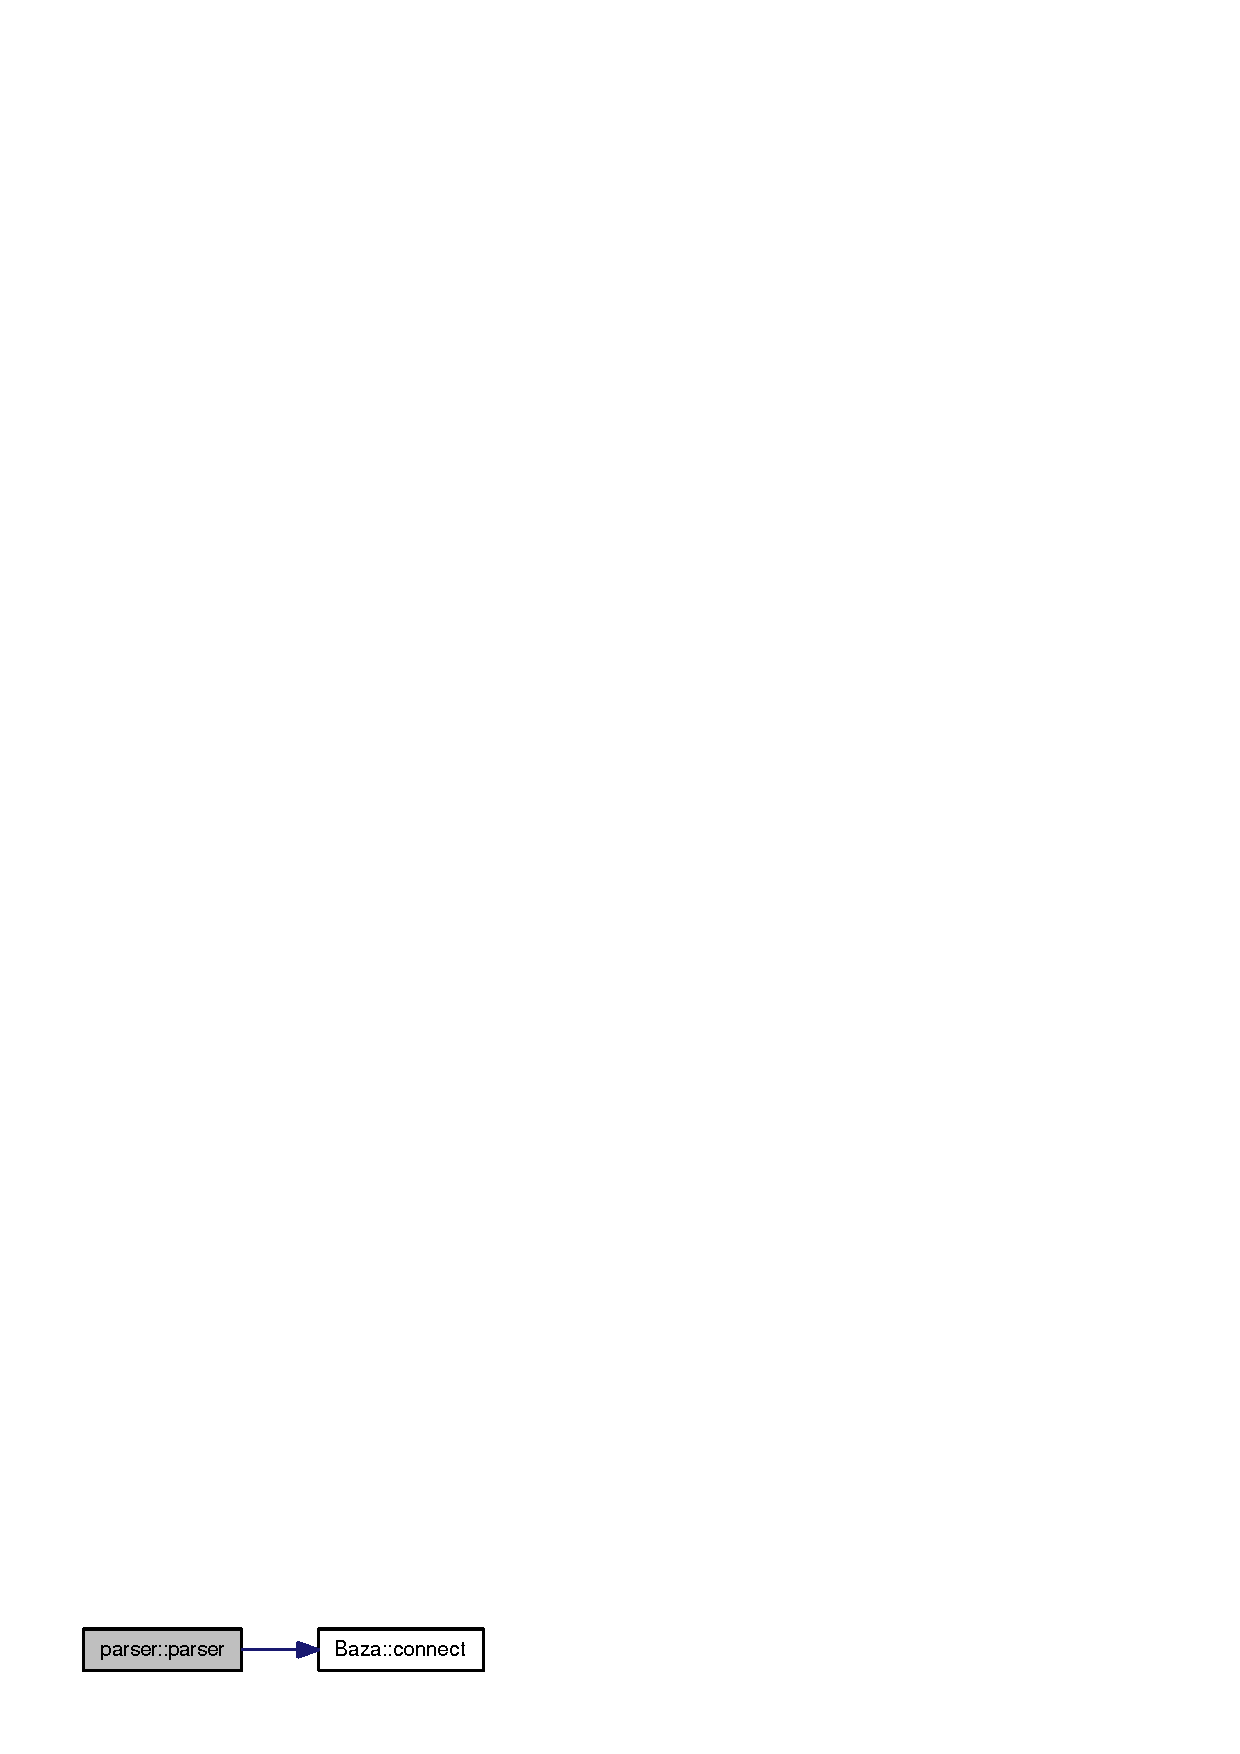
\includegraphics[width=118pt]{dd/dad/a00005_3a237071a3ab764cd61bc53df9dd4f46_cgraph}
\end{center}
\end{figure}


\subsection{Dokumentacja funkcji składowych}
\hypertarget{a00005_272ecc740702b4f48efdb8469b414b24}{
\index{parser@{parser}!czytanie\_\-z\_\-socketa@{czytanie\_\-z\_\-socketa}}
\index{czytanie\_\-z\_\-socketa@{czytanie\_\-z\_\-socketa}!parser@{parser}}
\subsubsection[{czytanie\_\-z\_\-socketa}]{\setlength{\rightskip}{0pt plus 5cm}std::string parser::czytanie\_\-z\_\-socketa ()\hspace{0.3cm}{\tt  \mbox{[}private\mbox{]}}}}
\label{dd/dad/a00005_272ecc740702b4f48efdb8469b414b24}


\hypertarget{a00005_96f941201d172eeaf2fb4d8429edfc0c}{
\index{parser@{parser}!lista\_\-plikow@{lista\_\-plikow}}
\index{lista\_\-plikow@{lista\_\-plikow}!parser@{parser}}
\subsubsection[{lista\_\-plikow}]{\setlength{\rightskip}{0pt plus 5cm}void parser::lista\_\-plikow (std::string {\em uzytkownik})\hspace{0.3cm}{\tt  \mbox{[}private\mbox{]}}}}
\label{dd/dad/a00005_96f941201d172eeaf2fb4d8429edfc0c}


Wysyła listę plików użytkownika 'uzytkownik'. 



Here is the caller graph for this function:\nopagebreak
\begin{figure}[H]
\begin{center}
\leavevmode
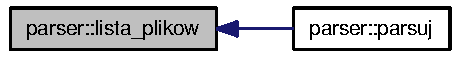
\includegraphics[width=128pt]{dd/dad/a00005_96f941201d172eeaf2fb4d8429edfc0c_icgraph}
\end{center}
\end{figure}
\hypertarget{a00005_71abf468eb72a833dbd6c8a895b66b52}{
\index{parser@{parser}!logowanie@{logowanie}}
\index{logowanie@{logowanie}!parser@{parser}}
\subsubsection[{logowanie}]{\setlength{\rightskip}{0pt plus 5cm}bool parser::logowanie (std::string {\em login}, \/  std::string {\em haslo})\hspace{0.3cm}{\tt  \mbox{[}private\mbox{]}}}}
\label{dd/dad/a00005_71abf468eb72a833dbd6c8a895b66b52}


Loguje klienta po przetworzeniu xmla odebranego od niego i sparsownaiu go w void \hyperlink{a00005_9ce7290217bd14e4efcbe2cad32ccf95}{parsuj()}. 



Here is the caller graph for this function:\nopagebreak
\begin{figure}[H]
\begin{center}
\leavevmode
\includegraphics[width=124pt]{dd/dad/a00005_71abf468eb72a833dbd6c8a895b66b52_icgraph}
\end{center}
\end{figure}
\hypertarget{a00005_4e084ae10e8498b171c44a0138597d2e}{
\index{parser@{parser}!odbieranie\_\-plikow@{odbieranie\_\-plikow}}
\index{odbieranie\_\-plikow@{odbieranie\_\-plikow}!parser@{parser}}
\subsubsection[{odbieranie\_\-plikow}]{\setlength{\rightskip}{0pt plus 5cm}void parser::odbieranie\_\-plikow (xmlpp::TextReader \& {\em reader}, \/  std::string {\em uzytkownik})\hspace{0.3cm}{\tt  \mbox{[}private\mbox{]}}}}
\label{dd/dad/a00005_4e084ae10e8498b171c44a0138597d2e}


Odbiera plik od użytkownika i umieszcza na serwerze. 



Here is the caller graph for this function:\nopagebreak
\begin{figure}[H]
\begin{center}
\leavevmode
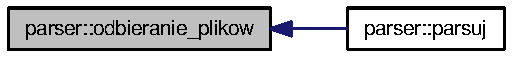
\includegraphics[width=141pt]{dd/dad/a00005_4e084ae10e8498b171c44a0138597d2e_icgraph}
\end{center}
\end{figure}
\hypertarget{a00005_e45404aec82f8c70a023bdc365c74287}{
\index{parser@{parser}!Odpowiedz@{Odpowiedz}}
\index{Odpowiedz@{Odpowiedz}!parser@{parser}}
\subsubsection[{Odpowiedz}]{\setlength{\rightskip}{0pt plus 5cm}void parser::Odpowiedz (int {\em nr\_\-odpowiedzi}, \/  int {\em nr\_\-operacji}, \/  std::string {\em odp})\hspace{0.3cm}{\tt  \mbox{[}private\mbox{]}}}}
\label{dd/dad/a00005_e45404aec82f8c70a023bdc365c74287}


Wysyła odpowiedź wielolinijkową zależnie od podanego i gdzie i jak w void \hyperlink{a00005_49d270636d2f3d5376c3cba62b5ea839}{Odpowiedz(int i, int numer\_\-operacji)};. 

\hypertarget{a00005_49d270636d2f3d5376c3cba62b5ea839}{
\index{parser@{parser}!Odpowiedz@{Odpowiedz}}
\index{Odpowiedz@{Odpowiedz}!parser@{parser}}
\subsubsection[{Odpowiedz}]{\setlength{\rightskip}{0pt plus 5cm}void parser::Odpowiedz (int {\em nr\_\-odpowiedzi}, \/  int {\em numer\_\-operacji} = {\tt -1})\hspace{0.3cm}{\tt  \mbox{[}private\mbox{]}}}}
\label{dd/dad/a00005_49d270636d2f3d5376c3cba62b5ea839}


Wysyła odpowiedź jednolinijkową zależnie od podanego i \begin{Desc}
\item[Parametry:]
\begin{description}
\item[{\em nr\_\-odpowiedzi}]Numer odpowiedzi 400 - bledne zapytanie 401 - bledny numer sesji 402 - podany plik istnieje (w przypadku wysylania pliku) 403 - wewnetrzny blad serwera 404 - podany plik nie istnieje 405 - błąd odbierania plikow 406 - wszystko OK \item[{\em numer\_\-operacji}]Numer operacji do której odnosi się podany nuemr odpowiedzi \end{description}
\end{Desc}


Here is the caller graph for this function:\nopagebreak
\begin{figure}[H]
\begin{center}
\leavevmode
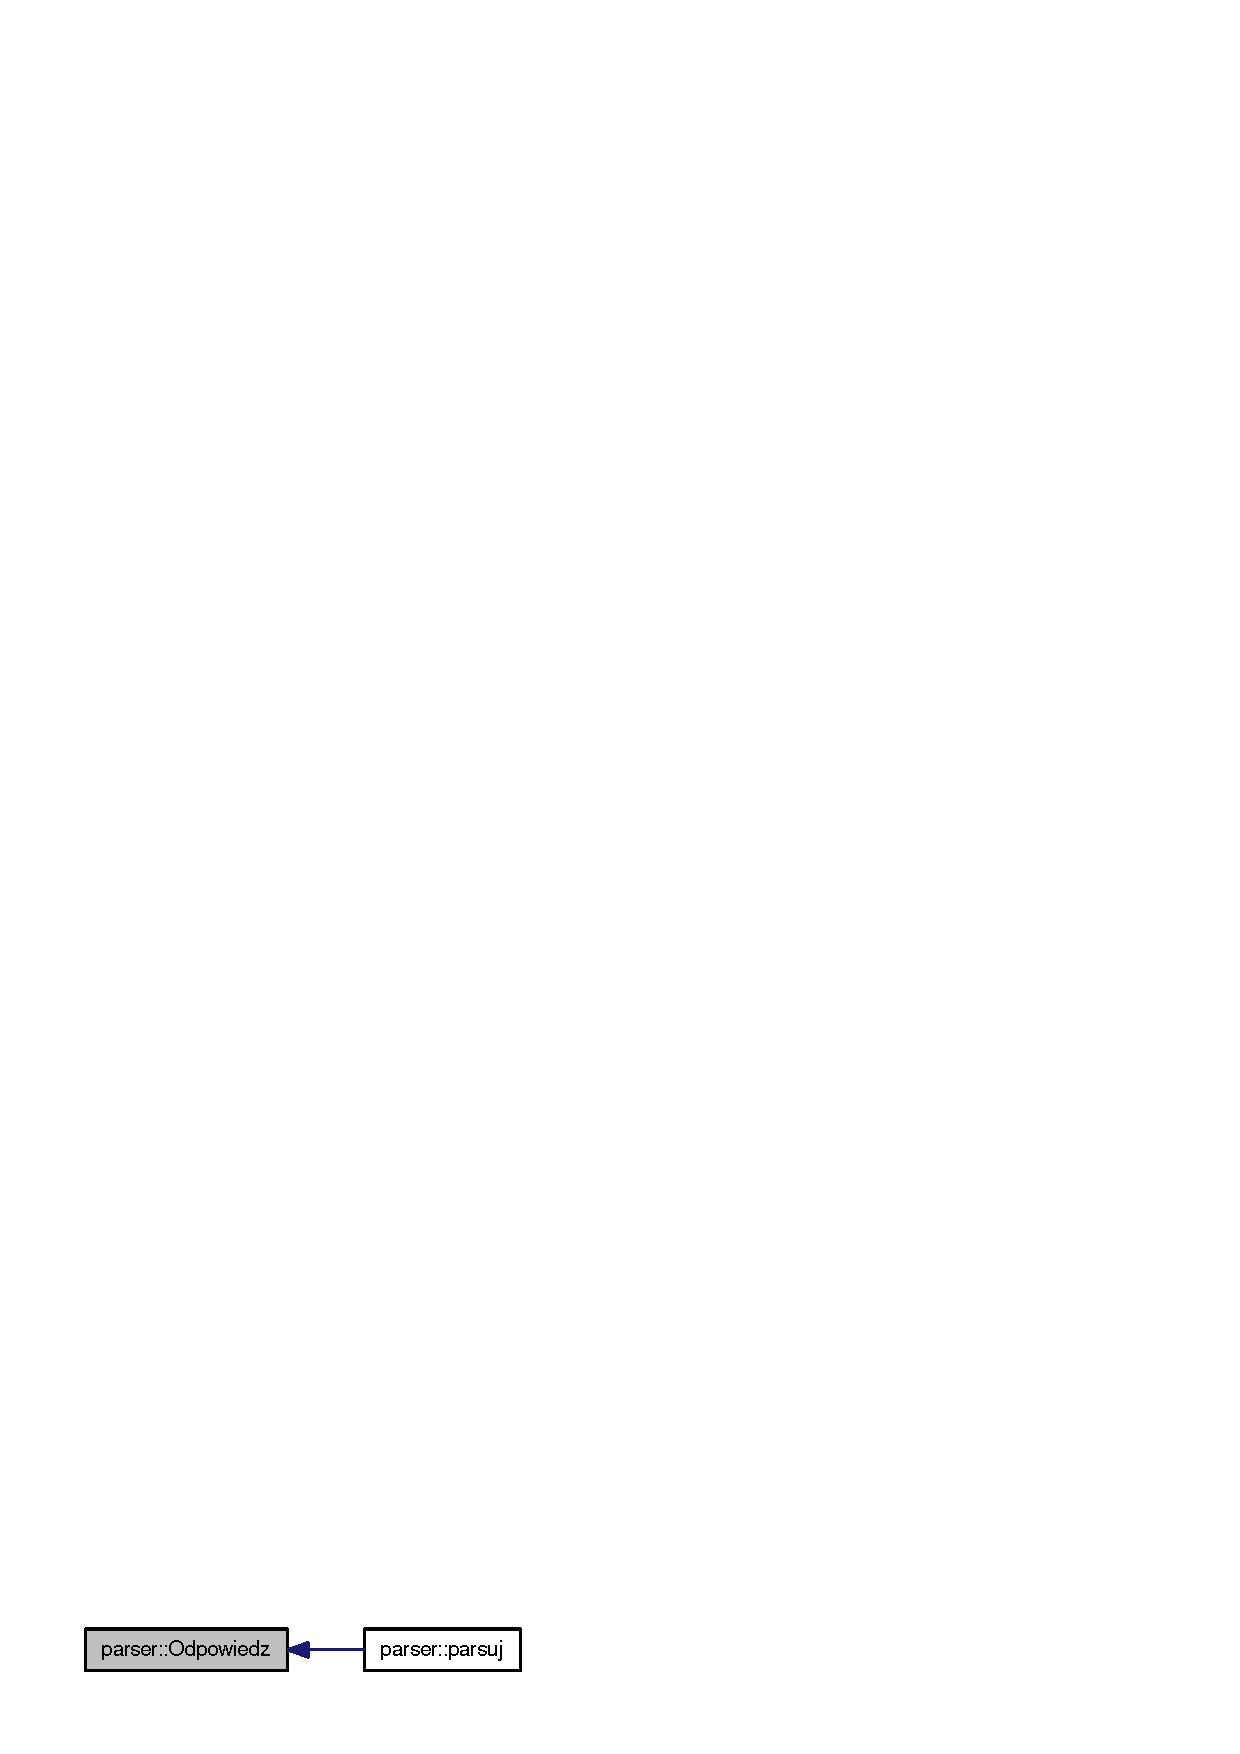
\includegraphics[width=127pt]{dd/dad/a00005_49d270636d2f3d5376c3cba62b5ea839_icgraph}
\end{center}
\end{figure}
\hypertarget{a00005_6a29174f787861caadc6c2e34b99f8c0}{
\index{parser@{parser}!odpowiedz\_\-login@{odpowiedz\_\-login}}
\index{odpowiedz\_\-login@{odpowiedz\_\-login}!parser@{parser}}
\subsubsection[{odpowiedz\_\-login}]{\setlength{\rightskip}{0pt plus 5cm}void parser::odpowiedz\_\-login (int {\em i})\hspace{0.3cm}{\tt  \mbox{[}private\mbox{]}}}}
\label{dd/dad/a00005_6a29174f787861caadc6c2e34b99f8c0}


Wysyła odpowiedź do logowania na podstawie podaneg i gdzie 0 - Logowanie przebieglo prawidlowo; 1 - błęde hasło lub login; 2 - nieoczekiwany błąd serwera; 3 - błędne zapytanie 

Here is the caller graph for this function:\nopagebreak
\begin{figure}[H]
\begin{center}
\leavevmode
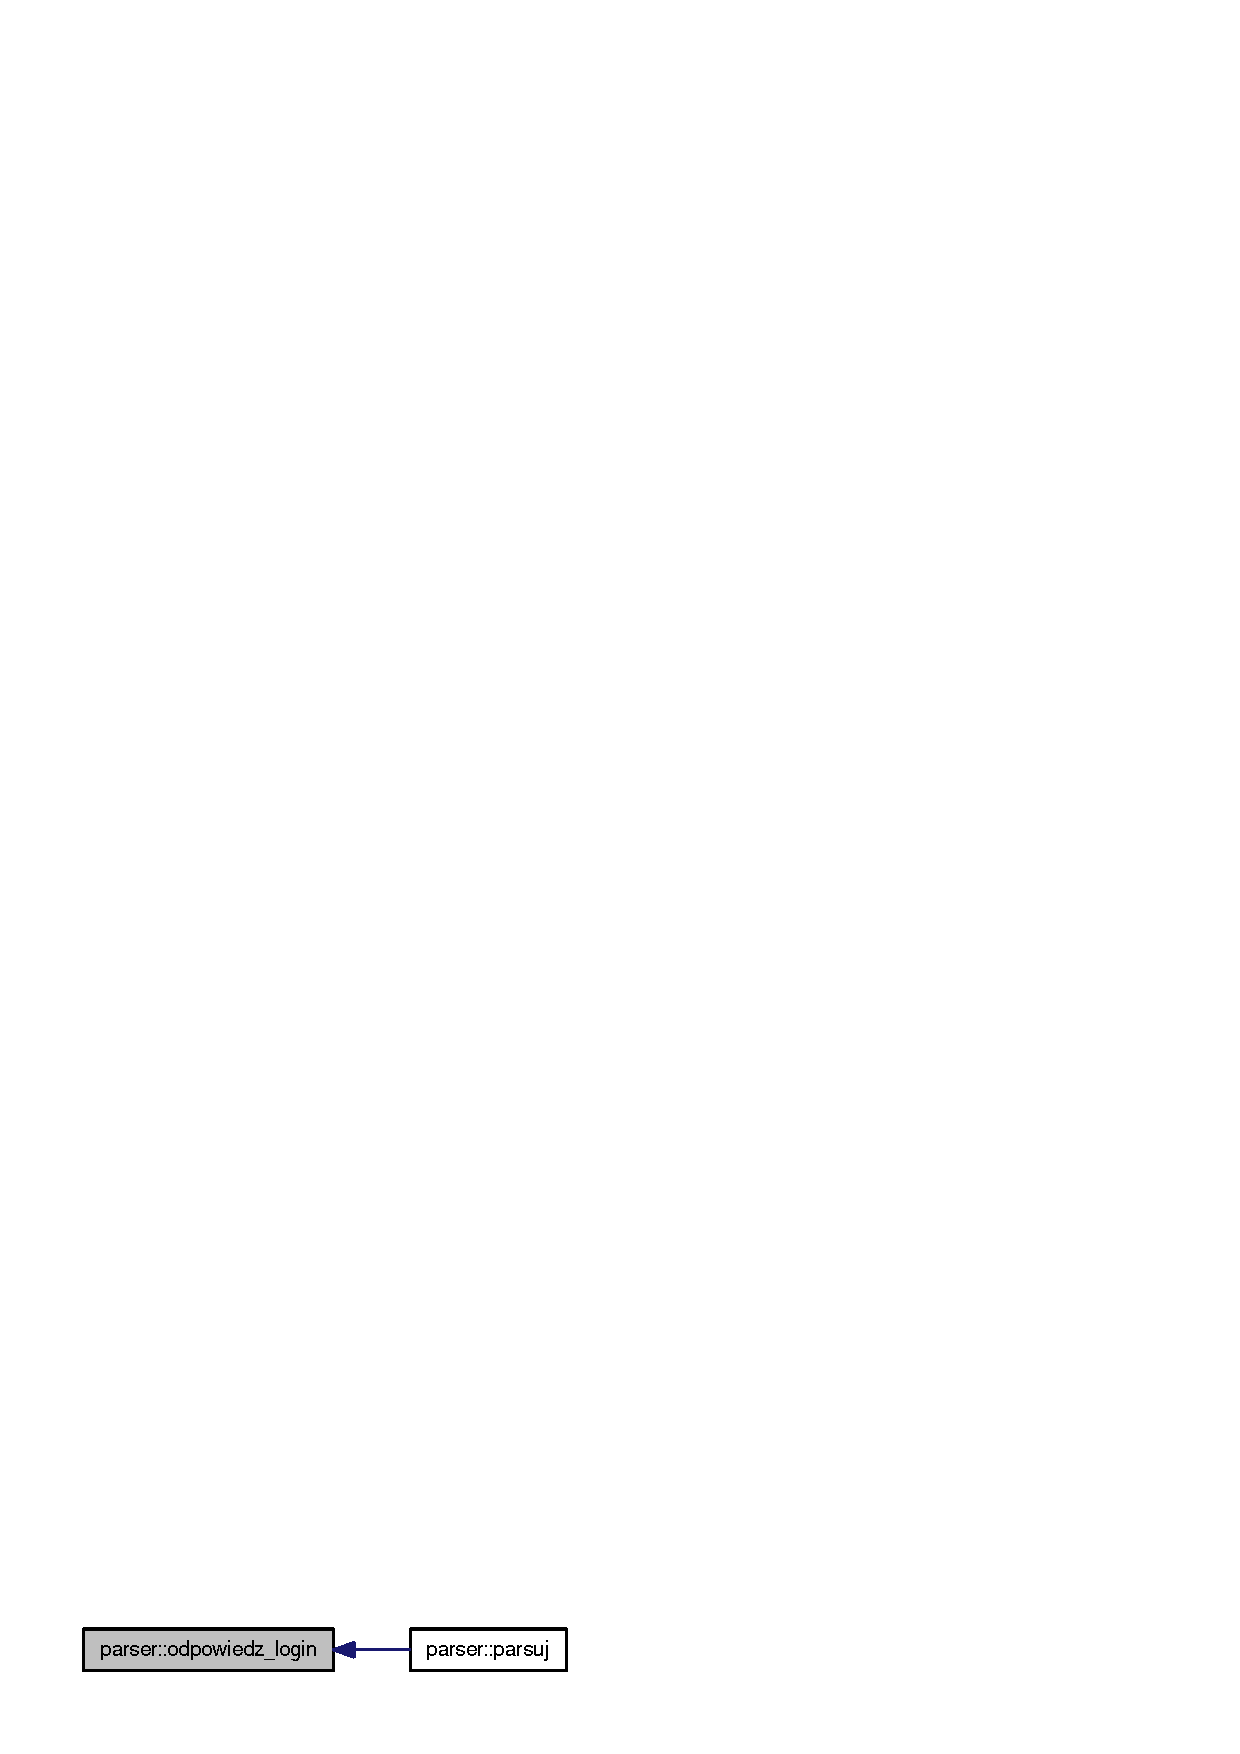
\includegraphics[width=138pt]{dd/dad/a00005_6a29174f787861caadc6c2e34b99f8c0_icgraph}
\end{center}
\end{figure}
\hypertarget{a00005_9ce7290217bd14e4efcbe2cad32ccf95}{
\index{parser@{parser}!parsuj@{parsuj}}
\index{parsuj@{parsuj}!parser@{parser}}
\subsubsection[{parsuj}]{\setlength{\rightskip}{0pt plus 5cm}bool parser::parsuj (std::string \& {\em do\_\-parsowania})\hspace{0.3cm}{\tt  \mbox{[}private\mbox{]}}}}
\label{dd/dad/a00005_9ce7290217bd14e4efcbe2cad32ccf95}


Parsuje dane pobrane od klienta. 



Logowanie - Trzeba pamiętać że \hyperlink{a00005}{parser} umieszcza dodatkowo spację na końcu sparsowanych stringów

Sprawdzanie ilosci atrybutów

Przesun sie do atrybutu \char`\"{}login\char`\"{}

Zapisz login

Gdy brak takiego atrybutu to konczymy rozmowe

Przesun sie do atrybutu \char`\"{}haslo\char`\"{}

Gdy brak takiego atrybutu to konczymy rozmowe

Sprawdzamy czy login i haslo pasują

Jeżeli tak to dajemy klientowi ID sesji

Jeżeli nie to informujemy go o tym i kończymy

Brak loginu i hasła

Jeżeli polecenie od klienta

Sprawdzanie ilosci atrybutów

Przesun sie do atrybutu \char`\"{}idsesji\char`\"{}

Sprawdzamy czy zgadza się id\_\-sesji

Sprawdzamy czy istnieje argument \char`\"{}operacja\char`\"{}

Błędne zapytanie

Niezgodne id\_\-sesji

Brak id\_\-sesji

Brak atrybutów

Funkcja wysyłająca dane przez SOCKET

Funkcja sprawdzająca czy dla podanego loginu hasło jest prawidłowe, jeżeli tak to generuje id\_\-sesji

Trzeba pamiętać że zmienna haslo tak naprawde zawiera haslo i na końcu spację.

Krotka odpowiedz gdzie i - kod odpowiedzi

Odpowiedź z dodatkowymi informacjami gdzie i - kod odpowiedzi

Funkcja wysyłająca odpowiedź po prośbie o zalogowanie

Funkcja wywoływana tylko raz, rozpoczyna pobieranie informacji z SOCKETA i przekazuje je parserowi

Jeżeli użytkownik to \char`\"{}.\char`\"{} to znaczy ze żadanie jest o liste plików użytkownika zalogowanego

Prośba o listę plików użytkownika uzytkownik 

Definicja w linii 16 pliku parser.cpp.

Oto graf wywołań dla tej funkcji:\nopagebreak
\begin{figure}[H]
\begin{center}
\leavevmode
\includegraphics[width=141pt]{dd/dad/a00005_9ce7290217bd14e4efcbe2cad32ccf95_cgraph}
\end{center}
\end{figure}
\hypertarget{a00005_05500b74ebdcc1578ead4c31fca73a5b}{
\index{parser@{parser}!pobieranie\_\-listy\_\-plikow@{pobieranie\_\-listy\_\-plikow}}
\index{pobieranie\_\-listy\_\-plikow@{pobieranie\_\-listy\_\-plikow}!parser@{parser}}
\subsubsection[{pobieranie\_\-listy\_\-plikow}]{\setlength{\rightskip}{0pt plus 5cm}std::vector$<$std::string$>$ parser::pobieranie\_\-listy\_\-plikow (xmlpp::TextReader \& {\em reader})\hspace{0.3cm}{\tt  \mbox{[}private\mbox{]}}}}
\label{dd/dad/a00005_05500b74ebdcc1578ead4c31fca73a5b}


Przygotowuje listę plikow do wysłania do klienta. 

\hypertarget{a00005_7793913f528921aa22c4b6cc259a0a14}{
\index{parser@{parser}!start@{start}}
\index{start@{start}!parser@{parser}}
\subsubsection[{start}]{\setlength{\rightskip}{0pt plus 5cm}void parser::start ()}}
\label{dd/dad/a00005_7793913f528921aa22c4b6cc259a0a14}




Here is the caller graph for this function:\nopagebreak
\begin{figure}[H]
\begin{center}
\leavevmode
\includegraphics[width=94pt]{dd/dad/a00005_7793913f528921aa22c4b6cc259a0a14_icgraph}
\end{center}
\end{figure}
\hypertarget{a00005_7ef79f818429f70b9cb35c0a33b59a10}{
\index{parser@{parser}!usun\_\-pliki@{usun\_\-pliki}}
\index{usun\_\-pliki@{usun\_\-pliki}!parser@{parser}}
\subsubsection[{usun\_\-pliki}]{\setlength{\rightskip}{0pt plus 5cm}void parser::usun\_\-pliki (xmlpp::TextReader \& {\em reader}, \/  std::string {\em uzytkownik})\hspace{0.3cm}{\tt  \mbox{[}private\mbox{]}}}}
\label{dd/dad/a00005_7ef79f818429f70b9cb35c0a33b59a10}


Usuwa plik z serwera (jeszcze nie zaimplementowane). 



Here is the caller graph for this function:\nopagebreak
\begin{figure}[H]
\begin{center}
\leavevmode
\includegraphics[width=125pt]{dd/dad/a00005_7ef79f818429f70b9cb35c0a33b59a10_icgraph}
\end{center}
\end{figure}
\hypertarget{a00005_2f6aceaa94a28fc699e4f824f7622b51}{
\index{parser@{parser}!wyslij@{wyslij}}
\index{wyslij@{wyslij}!parser@{parser}}
\subsubsection[{wyslij}]{\setlength{\rightskip}{0pt plus 5cm}void parser::wyslij (std::string {\em w})\hspace{0.3cm}{\tt  \mbox{[}private\mbox{]}}}}
\label{dd/dad/a00005_2f6aceaa94a28fc699e4f824f7622b51}


Wysyła dane podane w stringu w dodatkowo wysyłając znak końca linii. 



Here is the caller graph for this function:\nopagebreak
\begin{figure}[H]
\begin{center}
\leavevmode
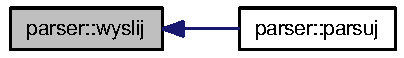
\includegraphics[width=115pt]{dd/dad/a00005_2f6aceaa94a28fc699e4f824f7622b51_icgraph}
\end{center}
\end{figure}
\hypertarget{a00005_771537f72f9e6a9cdb1d2961828eb66b}{
\index{parser@{parser}!wyslij\_\-plik@{wyslij\_\-plik}}
\index{wyslij\_\-plik@{wyslij\_\-plik}!parser@{parser}}
\subsubsection[{wyslij\_\-plik}]{\setlength{\rightskip}{0pt plus 5cm}void parser::wyslij\_\-plik (std::string {\em plik}, \/  std::string {\em uzytkownik})\hspace{0.3cm}{\tt  \mbox{[}private\mbox{]}}}}
\label{dd/dad/a00005_771537f72f9e6a9cdb1d2961828eb66b}


wysyła plik podany w argumencie 

\hypertarget{a00005_cc293df6220f5030fab5a7ee9cf8b1fa}{
\index{parser@{parser}!wysylanie\_\-plikow@{wysylanie\_\-plikow}}
\index{wysylanie\_\-plikow@{wysylanie\_\-plikow}!parser@{parser}}
\subsubsection[{wysylanie\_\-plikow}]{\setlength{\rightskip}{0pt plus 5cm}void parser::wysylanie\_\-plikow (xmlpp::TextReader \& {\em reader}, \/  std::string {\em uzytkownil})\hspace{0.3cm}{\tt  \mbox{[}private\mbox{]}}}}
\label{dd/dad/a00005_cc293df6220f5030fab5a7ee9cf8b1fa}


Odbiera od klienta informację jakie on chce pobrać pliki i przekazuje kazdy plik pojedynczo do \hyperlink{a00005_771537f72f9e6a9cdb1d2961828eb66b}{wyslij\_\-plik()}. 



Here is the caller graph for this function:\nopagebreak
\begin{figure}[H]
\begin{center}
\leavevmode
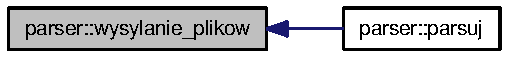
\includegraphics[width=140pt]{dd/dad/a00005_cc293df6220f5030fab5a7ee9cf8b1fa_icgraph}
\end{center}
\end{figure}


\subsection{Dokumentacja atrybutów składowych}
\hypertarget{a00005_21b4b313249353e48f7ea67f534ee519}{
\index{parser@{parser}!baza@{baza}}
\index{baza@{baza}!parser@{parser}}
\subsubsection[{baza}]{\setlength{\rightskip}{0pt plus 5cm}{\bf Baza} {\bf parser::baza}\hspace{0.3cm}{\tt  \mbox{[}private\mbox{]}}}}
\label{dd/dad/a00005_21b4b313249353e48f7ea67f534ee519}


Clasa obsługująca bazę danych. 



Definicja w linii 43 pliku parser.hpp.\hypertarget{a00005_2e7575bebca6d0fd9f5a8bfe6fc652d0}{
\index{parser@{parser}!bufor@{bufor}}
\index{bufor@{bufor}!parser@{parser}}
\subsubsection[{bufor}]{\setlength{\rightskip}{0pt plus 5cm}char {\bf parser::bufor}\mbox{[}BUFSIZE\mbox{]}\hspace{0.3cm}{\tt  \mbox{[}private\mbox{]}}}}
\label{dd/dad/a00005_2e7575bebca6d0fd9f5a8bfe6fc652d0}


Bufor danych. 



Definicja w linii 41 pliku parser.hpp.\hypertarget{a00005_2fc04d16e2ba688c5b306a2ad6770039}{
\index{parser@{parser}!haslo@{haslo}}
\index{haslo@{haslo}!parser@{parser}}
\subsubsection[{haslo}]{\setlength{\rightskip}{0pt plus 5cm}std::string {\bf parser::haslo}\hspace{0.3cm}{\tt  \mbox{[}private\mbox{]}}}}
\label{dd/dad/a00005_2fc04d16e2ba688c5b306a2ad6770039}


Zmienna przechowująca haslo (w przyszlosci hash hasla) uzytkownika. 



Definicja w linii 35 pliku parser.hpp.\hypertarget{a00005_aa8407d10d299b524fa2f74532e537ac}{
\index{parser@{parser}!id\_\-sesji@{id\_\-sesji}}
\index{id\_\-sesji@{id\_\-sesji}!parser@{parser}}
\subsubsection[{id\_\-sesji}]{\setlength{\rightskip}{0pt plus 5cm}int {\bf parser::id\_\-sesji}\hspace{0.3cm}{\tt  \mbox{[}private\mbox{]}}}}
\label{dd/dad/a00005_aa8407d10d299b524fa2f74532e537ac}


Aktualny ID sesji potrzebny pryz kazdym polaczneiu. 



Definicja w linii 39 pliku parser.hpp.\hypertarget{a00005_8bb124a2f285074773d1b0ee62cf0cc0}{
\index{parser@{parser}!login@{login}}
\index{login@{login}!parser@{parser}}
\subsubsection[{login}]{\setlength{\rightskip}{0pt plus 5cm}std::string {\bf parser::login}\hspace{0.3cm}{\tt  \mbox{[}private\mbox{]}}}}
\label{dd/dad/a00005_8bb124a2f285074773d1b0ee62cf0cc0}


Zmienna przechowująca login uzytkownika. 



Definicja w linii 33 pliku parser.hpp.\hypertarget{a00005_f95fb0cac229181329fa61f7bc72c65b}{
\index{parser@{parser}!stream@{stream}}
\index{stream@{stream}!parser@{parser}}
\subsubsection[{stream}]{\setlength{\rightskip}{0pt plus 5cm}tcp::iostream\& {\bf parser::stream}\hspace{0.3cm}{\tt  \mbox{[}private\mbox{]}}}}
\label{dd/dad/a00005_f95fb0cac229181329fa61f7bc72c65b}


Stream uzywany do odbierania i wysyłania informacji. 



Definicja w linii 31 pliku parser.hpp.

Dokumentacja dla tej klasy została wygenerowana z plików:\begin{CompactItemize}
\item 
/home/pawel/Dokumenty/Uczelnia/grupappz/Source/Ass8-server/\hyperlink{a00015}{parser.hpp}\item 
/home/pawel/Dokumenty/Uczelnia/grupappz/Source/Ass8-server/\hyperlink{a00014}{parser.cpp}\end{CompactItemize}

\hypertarget{a00006}{
\section{Dokumentacja pliku baza.cpp}
\label{de/d21/a00006}\index{baza.cpp@{baza.cpp}}
}
{\tt \#include \char`\"{}baza.hpp\char`\"{}}\par


Wykres zależności załączania dla baza.cpp:\nopagebreak
\begin{figure}[H]
\begin{center}
\leavevmode
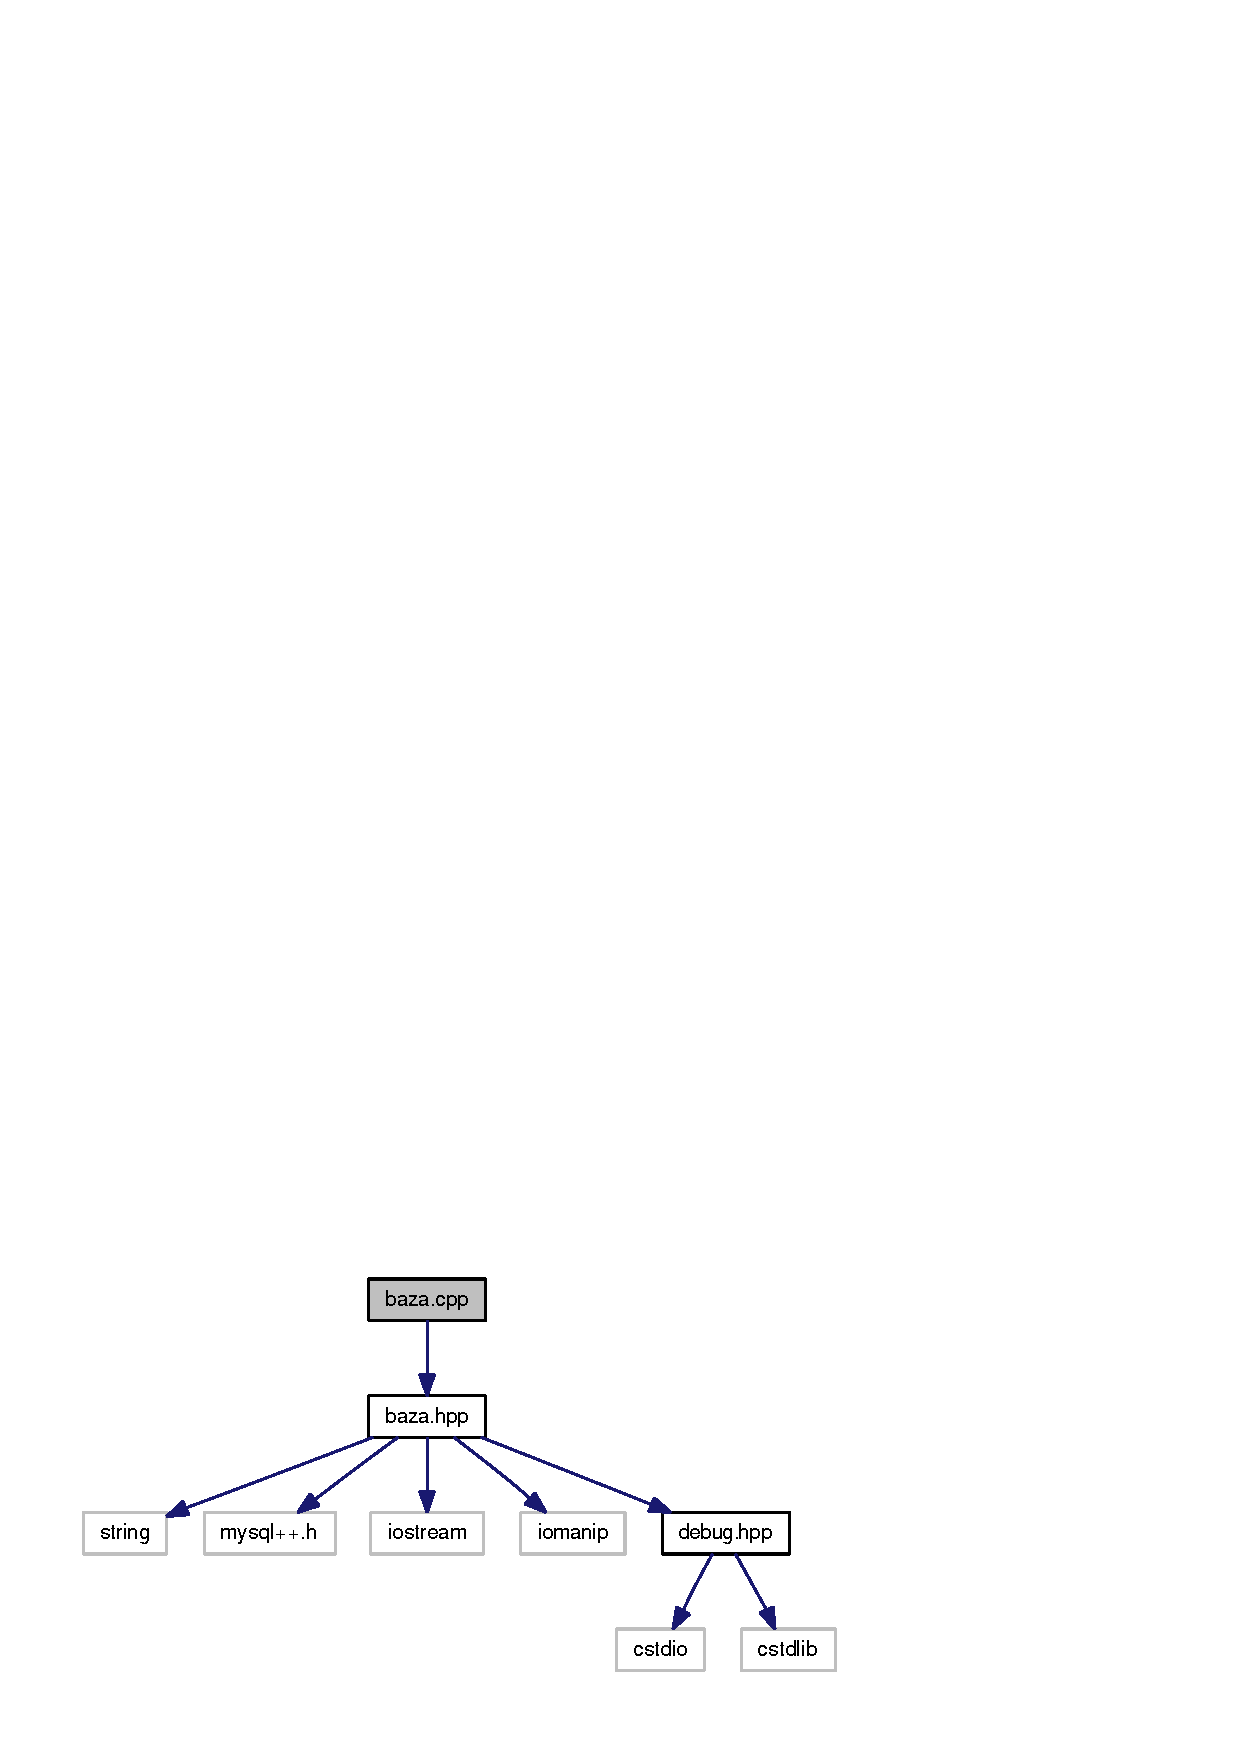
\includegraphics[width=202pt]{db/df3/a00034}
\end{center}
\end{figure}

\hypertarget{a00007}{
\section{Dokumentacja pliku baza.hpp}
\label{de/d5e/a00007}\index{baza.hpp@{baza.hpp}}
}
{\tt \#include $<$string$>$}\par
{\tt \#include $<$mysql++.h$>$}\par
{\tt \#include $<$iostream$>$}\par
{\tt \#include $<$iomanip$>$}\par
{\tt \#include \char`\"{}debug.hpp\char`\"{}}\par


Wykres zależności załączania dla baza.hpp:\nopagebreak
\begin{figure}[H]
\begin{center}
\leavevmode
\includegraphics[width=202pt]{d4/d8c/a00035}
\end{center}
\end{figure}


Ten wykres pokazuje, które pliki bezpośrednio lub pośrednio załączają ten plik:\nopagebreak
\begin{figure}[H]
\begin{center}
\leavevmode
\includegraphics[width=108pt]{de/d8c/a00036}
\end{center}
\end{figure}
\subsection*{Komponenty}
\begin{CompactItemize}
\item 
class \hyperlink{a00001}{Baza}
\end{CompactItemize}

\hypertarget{a00008}{
\section{Dokumentacja pliku /home/pawel/Dokumenty/Uczelnia/grupappz/Source/Ass8-server/parser.hpp}
\label{a00008}\index{/home/pawel/Dokumenty/Uczelnia/grupappz/Source/Ass8-server/parser.hpp@{/home/pawel/Dokumenty/Uczelnia/grupappz/Source/Ass8-server/parser.hpp}}
}
{\tt \#include $<$boost/asio.hpp$>$}\par
{\tt \#include $<$string$>$}\par
{\tt \#include $<$fstream$>$}\par
{\tt \#include $<$libxml++/libxml++.h$>$}\par
{\tt \#include $<$libxml++/parsers/textreader.h$>$}\par
{\tt \#include \char`\"{}baza.hpp\char`\"{}}\par
{\tt \#include \char`\"{}debug.hpp\char`\"{}}\par


Wykres zależności załączania dla parser.hpp:\nopagebreak
\begin{figure}[H]
\begin{center}
\leavevmode
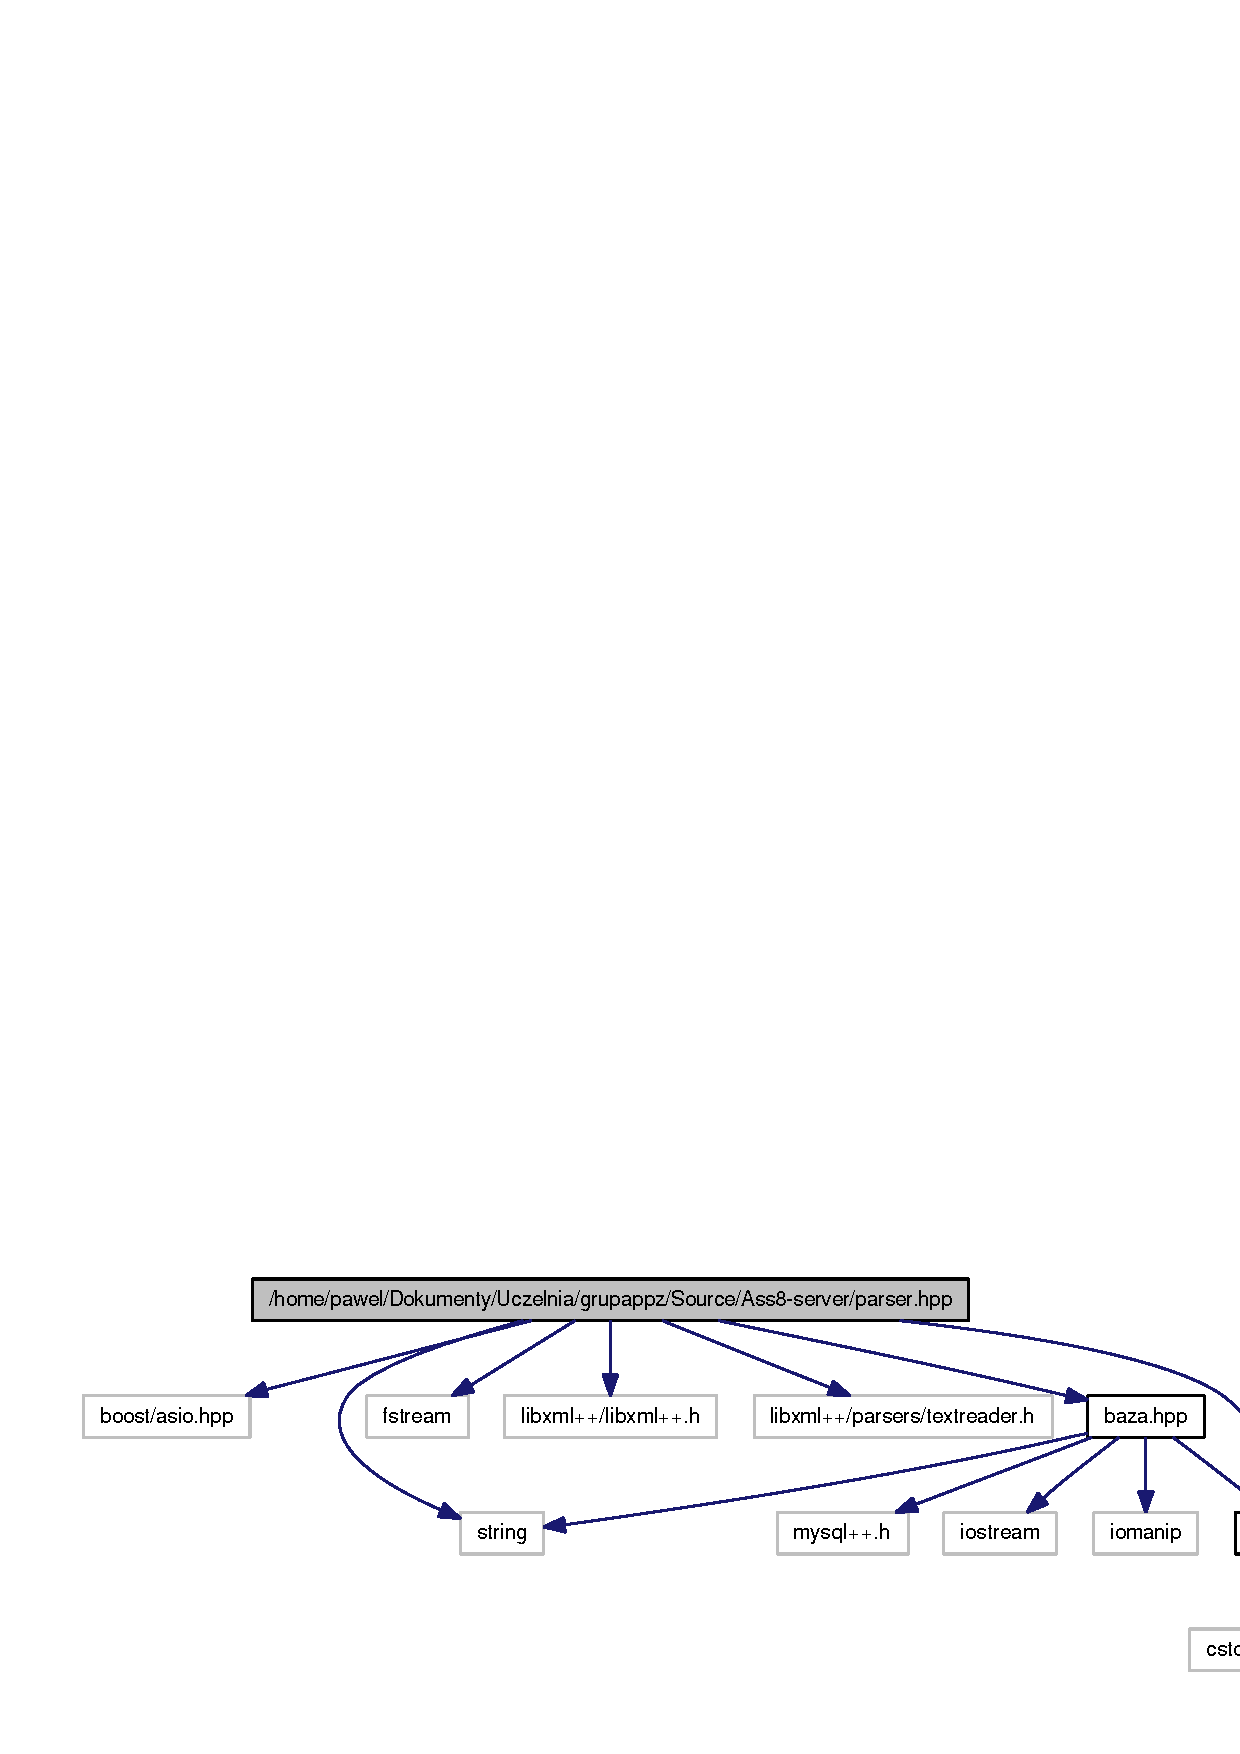
\includegraphics[width=339pt]{a00030}
\end{center}
\end{figure}


Ten wykres pokazuje, które pliki bezpośrednio lub pośrednio załączają ten plik:\nopagebreak
\begin{figure}[H]
\begin{center}
\leavevmode
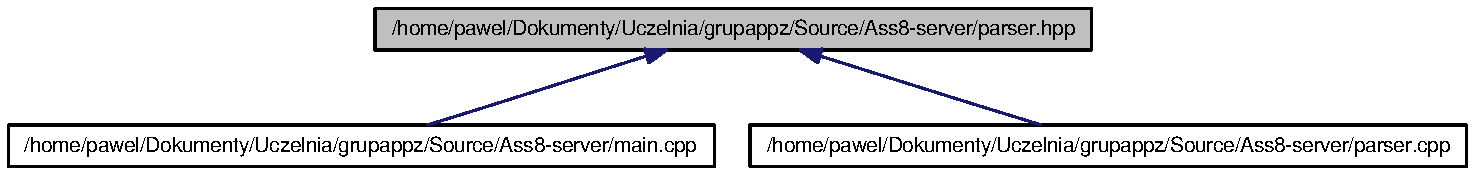
\includegraphics[width=372pt]{a00031}
\end{center}
\end{figure}
\subsection*{Komponenty}
\begin{CompactItemize}
\item 
class \hyperlink{a00002}{parser}
\end{CompactItemize}
\subsection*{Definicje}
\begin{CompactItemize}
\item 
\#define \hyperlink{a00008_eca034f67218340ecb2261a22c2f3dcd}{BUFSIZE}~1024
\item 
\#define \hyperlink{a00008_b46db07bcc5d1bb3dbc73f7be2592ee0}{BUFSIZE2}~1024$\ast$2
\end{CompactItemize}
\subsection*{Funkcje}
\begin{CompactItemize}
\item 
void \hyperlink{a00008_6c724feff242ad0cd599cdd458f73199}{eat\_\-zombie} ()
\end{CompactItemize}


\subsection{Dokumentacja definicji}
\hypertarget{a00008_eca034f67218340ecb2261a22c2f3dcd}{
\index{parser.hpp@{parser.hpp}!BUFSIZE@{BUFSIZE}}
\index{BUFSIZE@{BUFSIZE}!parser.hpp@{parser.hpp}}
\subsubsection[{BUFSIZE}]{\setlength{\rightskip}{0pt plus 5cm}\#define BUFSIZE~1024}}
\label{a00008_eca034f67218340ecb2261a22c2f3dcd}




Definicja w linii 19 pliku parser.hpp.\hypertarget{a00008_b46db07bcc5d1bb3dbc73f7be2592ee0}{
\index{parser.hpp@{parser.hpp}!BUFSIZE2@{BUFSIZE2}}
\index{BUFSIZE2@{BUFSIZE2}!parser.hpp@{parser.hpp}}
\subsubsection[{BUFSIZE2}]{\setlength{\rightskip}{0pt plus 5cm}\#define BUFSIZE2~1024$\ast$2}}
\label{a00008_b46db07bcc5d1bb3dbc73f7be2592ee0}




Definicja w linii 20 pliku parser.hpp.

\subsection{Dokumentacja funkcji}
\hypertarget{a00008_6c724feff242ad0cd599cdd458f73199}{
\index{parser.hpp@{parser.hpp}!eat\_\-zombie@{eat\_\-zombie}}
\index{eat\_\-zombie@{eat\_\-zombie}!parser.hpp@{parser.hpp}}
\subsubsection[{eat\_\-zombie}]{\setlength{\rightskip}{0pt plus 5cm}void eat\_\-zombie ()}}
\label{a00008_6c724feff242ad0cd599cdd458f73199}




Here is the caller graph for this function:\nopagebreak
\begin{figure}[H]
\begin{center}
\leavevmode
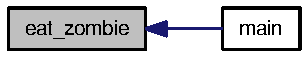
\includegraphics[width=92pt]{a00008_6c724feff242ad0cd599cdd458f73199_icgraph}
\end{center}
\end{figure}

\hypertarget{a00009}{
\section{Dokumentacja klasy ASS8.Klient.klientLogowanie}
\label{da/da0/a00009}\index{ASS8::Klient::klientLogowanie@{ASS8::Klient::klientLogowanie}}
}
Klasa zawiera dane do serializacji zapytania o logowanie.  


\subsection*{Metody publiczne}
\begin{CompactItemize}
\item 
\hyperlink{a00009_35b35cead7d9f58a9c114ca328012f32}{klientLogowanie} ()
\item 
\hyperlink{a00009_be81e6b3b3e980fc92672d677ee97602}{klientLogowanie} (string l, string h, string v)
\end{CompactItemize}
\subsection*{Właściwości}
\begin{CompactItemize}
\item 
string \hyperlink{a00009_bf20831d9b7c79f4c9de90320ff7e250}{Login}\hspace{0.3cm}{\tt  \mbox{[}get, set\mbox{]}}
\item 
string \hyperlink{a00009_6f3c62f8e9b616f4b214788974fe93cd}{Haslo}\hspace{0.3cm}{\tt  \mbox{[}get, set\mbox{]}}
\item 
string \hyperlink{a00009_aa3348ed5721633094699e4ab4b43289}{wersjaKlienta}\hspace{0.3cm}{\tt  \mbox{[}get, set\mbox{]}}
\end{CompactItemize}
\subsection*{Atrybuty prywatne}
\begin{CompactItemize}
\item 
string \hyperlink{a00009_1fa00149f1a375887302be1b66d76f51}{login}
\item 
string \hyperlink{a00009_ee8fc634a45d3b1c48c0fda5de62aa8b}{haslo}
\item 
string \hyperlink{a00009_4f1ccf1f388e4f7c412a91ceefd11cc8}{vKlienta}
\end{CompactItemize}


\subsection{Opis szczegółowy}
Klasa zawiera dane do serializacji zapytania o logowanie. 



Definicja w linii 145 pliku XmlRequestsClass.cs.

\subsection{Dokumentacja konstruktora i destruktora}
\hypertarget{a00009_35b35cead7d9f58a9c114ca328012f32}{
\index{ASS8::Klient::klientLogowanie@{ASS8::Klient::klientLogowanie}!klientLogowanie@{klientLogowanie}}
\index{klientLogowanie@{klientLogowanie}!ASS8::Klient::klientLogowanie@{ASS8::Klient::klientLogowanie}}
\subsubsection[{klientLogowanie}]{\setlength{\rightskip}{0pt plus 5cm}ASS8.Klient.klientLogowanie.klientLogowanie ()}}
\label{da/da0/a00009_35b35cead7d9f58a9c114ca328012f32}




Definicja w linii 147 pliku XmlRequestsClass.cs.\hypertarget{a00009_be81e6b3b3e980fc92672d677ee97602}{
\index{ASS8::Klient::klientLogowanie@{ASS8::Klient::klientLogowanie}!klientLogowanie@{klientLogowanie}}
\index{klientLogowanie@{klientLogowanie}!ASS8::Klient::klientLogowanie@{ASS8::Klient::klientLogowanie}}
\subsubsection[{klientLogowanie}]{\setlength{\rightskip}{0pt plus 5cm}ASS8.Klient.klientLogowanie.klientLogowanie (string {\em l}, \/  string {\em h}, \/  string {\em v})}}
\label{da/da0/a00009_be81e6b3b3e980fc92672d677ee97602}




Definicja w linii 148 pliku XmlRequestsClass.cs.

\subsection{Dokumentacja atrybutów składowych}
\hypertarget{a00009_ee8fc634a45d3b1c48c0fda5de62aa8b}{
\index{ASS8::Klient::klientLogowanie@{ASS8::Klient::klientLogowanie}!haslo@{haslo}}
\index{haslo@{haslo}!ASS8::Klient::klientLogowanie@{ASS8::Klient::klientLogowanie}}
\subsubsection[{haslo}]{\setlength{\rightskip}{0pt plus 5cm}string {\bf ASS8.Klient.klientLogowanie.haslo}\hspace{0.3cm}{\tt  \mbox{[}private\mbox{]}}}}
\label{da/da0/a00009_ee8fc634a45d3b1c48c0fda5de62aa8b}




Definicja w linii 192 pliku XmlRequestsClass.cs.\hypertarget{a00009_1fa00149f1a375887302be1b66d76f51}{
\index{ASS8::Klient::klientLogowanie@{ASS8::Klient::klientLogowanie}!login@{login}}
\index{login@{login}!ASS8::Klient::klientLogowanie@{ASS8::Klient::klientLogowanie}}
\subsubsection[{login}]{\setlength{\rightskip}{0pt plus 5cm}string {\bf ASS8.Klient.klientLogowanie.login}\hspace{0.3cm}{\tt  \mbox{[}private\mbox{]}}}}
\label{da/da0/a00009_1fa00149f1a375887302be1b66d76f51}




Definicja w linii 191 pliku XmlRequestsClass.cs.\hypertarget{a00009_4f1ccf1f388e4f7c412a91ceefd11cc8}{
\index{ASS8::Klient::klientLogowanie@{ASS8::Klient::klientLogowanie}!vKlienta@{vKlienta}}
\index{vKlienta@{vKlienta}!ASS8::Klient::klientLogowanie@{ASS8::Klient::klientLogowanie}}
\subsubsection[{vKlienta}]{\setlength{\rightskip}{0pt plus 5cm}string {\bf ASS8.Klient.klientLogowanie.vKlienta}\hspace{0.3cm}{\tt  \mbox{[}private\mbox{]}}}}
\label{da/da0/a00009_4f1ccf1f388e4f7c412a91ceefd11cc8}




Definicja w linii 193 pliku XmlRequestsClass.cs.

\subsection{Dokumentacja właściwości}
\hypertarget{a00009_6f3c62f8e9b616f4b214788974fe93cd}{
\index{ASS8::Klient::klientLogowanie@{ASS8::Klient::klientLogowanie}!Haslo@{Haslo}}
\index{Haslo@{Haslo}!ASS8::Klient::klientLogowanie@{ASS8::Klient::klientLogowanie}}
\subsubsection[{Haslo}]{\setlength{\rightskip}{0pt plus 5cm}string ASS8.Klient.klientLogowanie.Haslo\hspace{0.3cm}{\tt  \mbox{[}get, set\mbox{]}}}}
\label{da/da0/a00009_6f3c62f8e9b616f4b214788974fe93cd}




Definicja w linii 168 pliku XmlRequestsClass.cs.\hypertarget{a00009_bf20831d9b7c79f4c9de90320ff7e250}{
\index{ASS8::Klient::klientLogowanie@{ASS8::Klient::klientLogowanie}!Login@{Login}}
\index{Login@{Login}!ASS8::Klient::klientLogowanie@{ASS8::Klient::klientLogowanie}}
\subsubsection[{Login}]{\setlength{\rightskip}{0pt plus 5cm}string ASS8.Klient.klientLogowanie.Login\hspace{0.3cm}{\tt  \mbox{[}get, set\mbox{]}}}}
\label{da/da0/a00009_bf20831d9b7c79f4c9de90320ff7e250}




Definicja w linii 156 pliku XmlRequestsClass.cs.\hypertarget{a00009_aa3348ed5721633094699e4ab4b43289}{
\index{ASS8::Klient::klientLogowanie@{ASS8::Klient::klientLogowanie}!wersjaKlienta@{wersjaKlienta}}
\index{wersjaKlienta@{wersjaKlienta}!ASS8::Klient::klientLogowanie@{ASS8::Klient::klientLogowanie}}
\subsubsection[{wersjaKlienta}]{\setlength{\rightskip}{0pt plus 5cm}string ASS8.Klient.klientLogowanie.wersjaKlienta\hspace{0.3cm}{\tt  \mbox{[}get, set\mbox{]}}}}
\label{da/da0/a00009_aa3348ed5721633094699e4ab4b43289}




Definicja w linii 180 pliku XmlRequestsClass.cs.

Dokumentacja dla tej klasy została wygenerowana z pliku:\begin{CompactItemize}
\item 
\hyperlink{a00055}{XmlRequestsClass.cs}\end{CompactItemize}

\hypertarget{a00010}{
\section{Dokumentacja pliku md5.cpp}
\label{d7/dec/a00010}\index{md5.cpp@{md5.cpp}}
}
{\tt \#include \char`\"{}md5.h\char`\"{}}\par


Wykres zależności załączania dla md5.cpp:\nopagebreak
\begin{figure}[H]
\begin{center}
\leavevmode
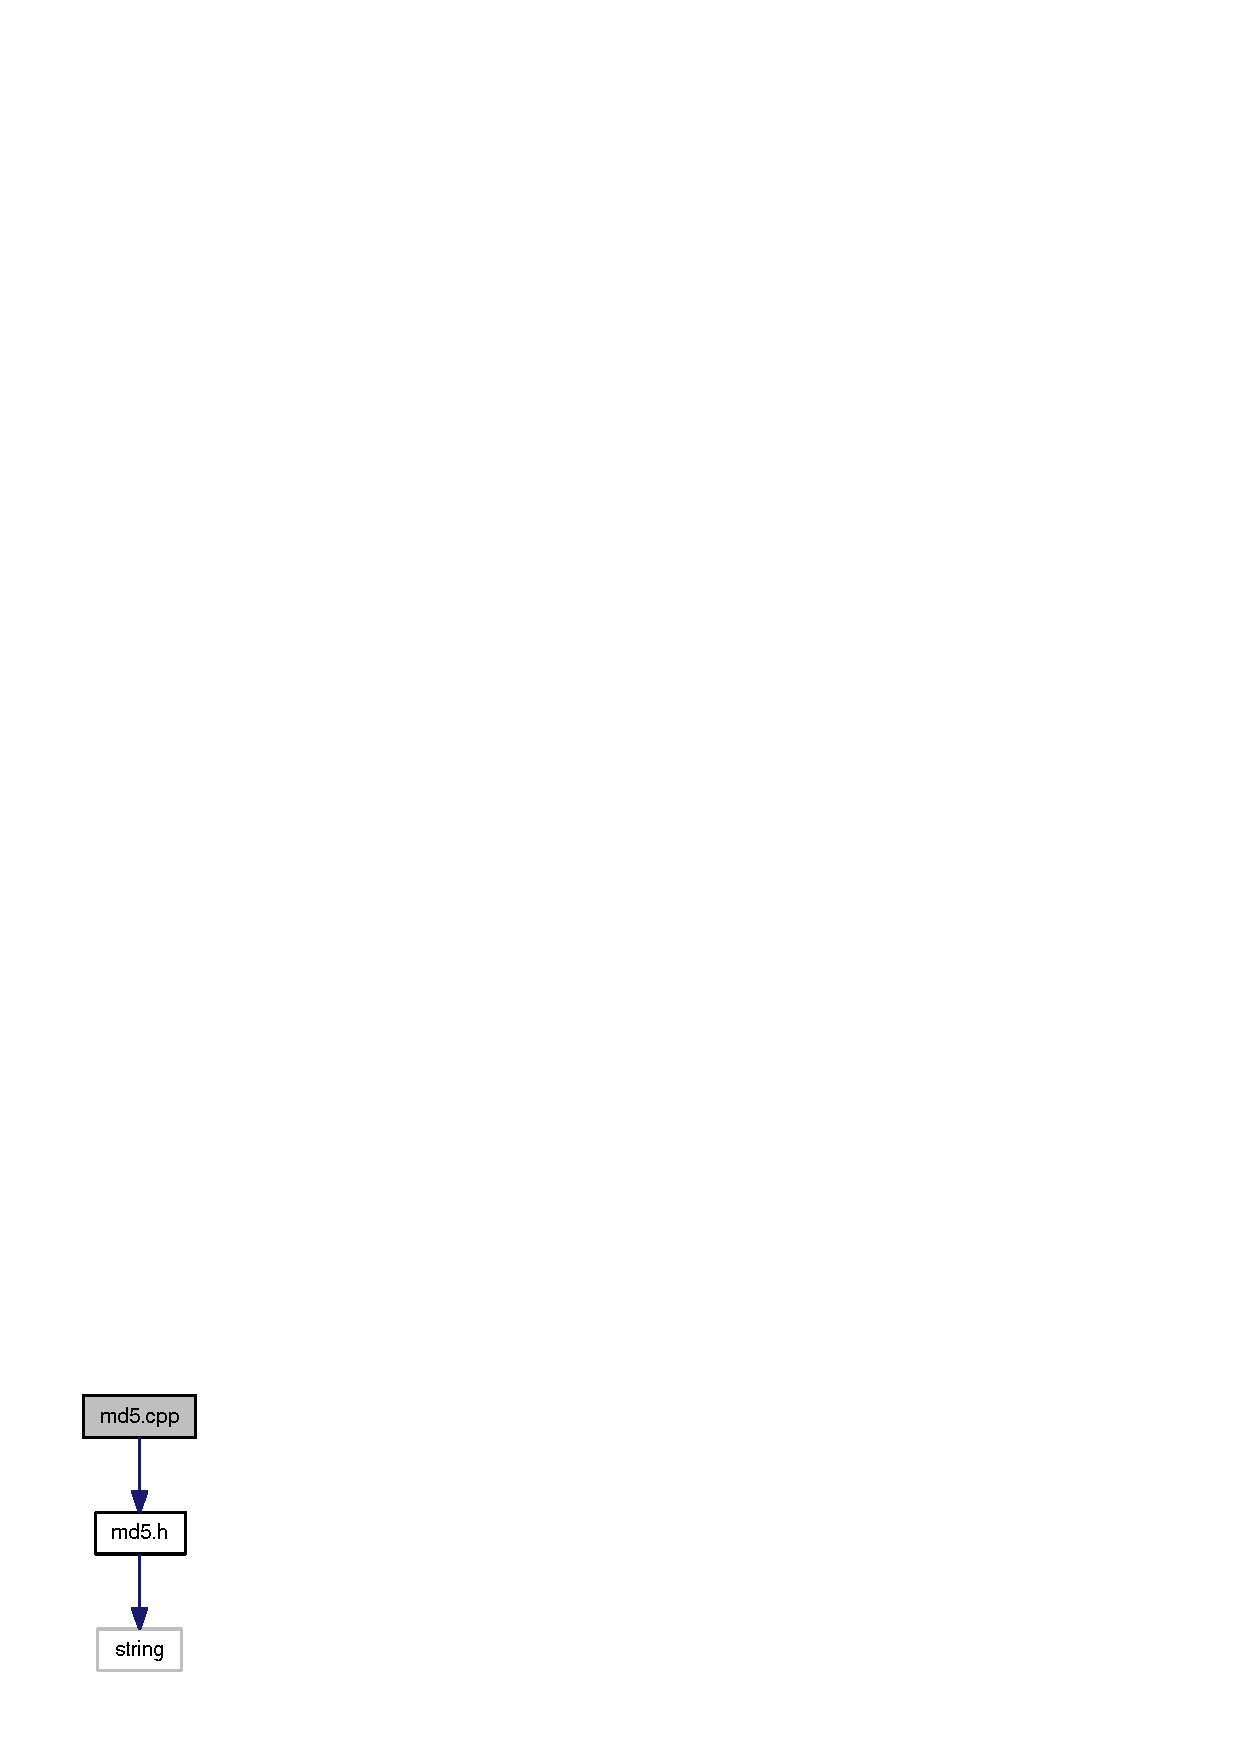
\includegraphics[width=49pt]{dd/d32/a00041}
\end{center}
\end{figure}
\subsection*{Definicje}
\begin{CompactItemize}
\item 
\#define \hyperlink{a00010_51398c0e5541164ad4d6615880073305}{S11}~7
\item 
\#define \hyperlink{a00010_1ec499cd0e54ecc28c2ac2afea5b038e}{S12}~12
\item 
\#define \hyperlink{a00010_aeec90429105fb54d853dd4fc7027a54}{S13}~17
\item 
\#define \hyperlink{a00010_78342b0ccde2ed12fdf19a113cc266cf}{S14}~22
\item 
\#define \hyperlink{a00010_b6d5354f647a0e7592a1f051fc8377b2}{S21}~5
\item 
\#define \hyperlink{a00010_ddad30455da936bc1879ee9c72b46d59}{S22}~9
\item 
\#define \hyperlink{a00010_6321a8b29628936f76e9e78cf5bda95f}{S23}~14
\item 
\#define \hyperlink{a00010_0c09eb77d30a0d5f9154914147b86c20}{S24}~20
\item 
\#define \hyperlink{a00010_ef26590f8a880ee6f4a158168defcd89}{S31}~4
\item 
\#define \hyperlink{a00010_1d512424dd8a91e0a5bcc98563f33914}{S32}~11
\item 
\#define \hyperlink{a00010_1c854214533f6220e859b0063196abb3}{S33}~16
\item 
\#define \hyperlink{a00010_f6472be1d535970afee8e5266a74aa07}{S34}~23
\item 
\#define \hyperlink{a00010_b674ba129e588da55d1d494e1cf3c15e}{S41}~6
\item 
\#define \hyperlink{a00010_268ef1a49114a94b931cc6b313e3cd1b}{S42}~10
\item 
\#define \hyperlink{a00010_5aaa7121f39650d472746942ca68f959}{S43}~15
\item 
\#define \hyperlink{a00010_6a3989af72b55d169bd73a66f8620aae}{S44}~21
\item 
\#define \hyperlink{a00010_96d73bbd7af15cb1fc38c3f4a3bd82e9}{F}(x, y, z)~(((x) \& (y)) $|$ (($\sim$x) \& (z)))
\item 
\#define \hyperlink{a00010_d96b7cf3182ce2ba85e5a7a93b12c441}{G}(x, y, z)~(((x) \& (z)) $|$ ((y) \& ($\sim$z)))
\item 
\#define \hyperlink{a00010_e42219072d798876e6b08e6b78614ff6}{H}(x, y, z)~((x) $^\wedge$ (y) $^\wedge$ (z))
\item 
\#define \hyperlink{a00010_c0eafdc9ee161b71e7af98af736952fd}{I}(x, y, z)~((y) $^\wedge$ ((x) $|$ ($\sim$z)))
\item 
\#define \hyperlink{a00010_7417fd4e875360c0533fa5b412cdab49}{ROTATE\_\-LEFT}(x, n)~(((x) $<$$<$ (n)) $|$ ((x) $>$$>$ (32-(n))))
\item 
\#define \hyperlink{a00010_0a143972cb6c4fe16f0ffa8a3d41ebf3}{FF}(a, b, c, d, x, s, ac)
\item 
\#define \hyperlink{a00010_685f32faa2a66e743850b990a13b8bfa}{GG}(a, b, c, d, x, s, ac)
\item 
\#define \hyperlink{a00010_8b9f1c4778df01ef970b87dbe5541dc5}{HH}(a, b, c, d, x, s, ac)
\item 
\#define \hyperlink{a00010_d26626e5efb37b2dadef4e88e35e4329}{II}(a, b, c, d, x, s, ac)
\end{CompactItemize}
\subsection*{Zmienne}
\begin{CompactItemize}
\item 
static unsigned char \hyperlink{a00010_ee6f420120b0fbc0fb096cb61655cec4}{PADDING} \mbox{[}64\mbox{]}
\end{CompactItemize}


\subsection{Dokumentacja definicji}
\hypertarget{a00010_96d73bbd7af15cb1fc38c3f4a3bd82e9}{
\index{md5.cpp@{md5.cpp}!F@{F}}
\index{F@{F}!md5.cpp@{md5.cpp}}
\subsubsection[{F}]{\setlength{\rightskip}{0pt plus 5cm}\#define F(x, \/  y, \/  z)~(((x) \& (y)) $|$ (($\sim$x) \& (z)))}}
\label{d7/dec/a00010_96d73bbd7af15cb1fc38c3f4a3bd82e9}




Definicja w linii 62 pliku md5.cpp.\hypertarget{a00010_0a143972cb6c4fe16f0ffa8a3d41ebf3}{
\index{md5.cpp@{md5.cpp}!FF@{FF}}
\index{FF@{FF}!md5.cpp@{md5.cpp}}
\subsubsection[{FF}]{\setlength{\rightskip}{0pt plus 5cm}\#define FF(a, \/  b, \/  c, \/  d, \/  x, \/  s, \/  ac)}}
\label{d7/dec/a00010_0a143972cb6c4fe16f0ffa8a3d41ebf3}


\textbf{Wartość:}

\begin{Code}\begin{verbatim}{ \
 (a) += F ((b), (c), (d)) + (x) + (unsigned long int)(ac); \
 (a) = ROTATE_LEFT ((a), (s)); \
 (a) += (b); \
  }
\end{verbatim}
\end{Code}


Definicja w linii 75 pliku md5.cpp.\hypertarget{a00010_d96b7cf3182ce2ba85e5a7a93b12c441}{
\index{md5.cpp@{md5.cpp}!G@{G}}
\index{G@{G}!md5.cpp@{md5.cpp}}
\subsubsection[{G}]{\setlength{\rightskip}{0pt plus 5cm}\#define G(x, \/  y, \/  z)~(((x) \& (z)) $|$ ((y) \& ($\sim$z)))}}
\label{d7/dec/a00010_d96b7cf3182ce2ba85e5a7a93b12c441}




Definicja w linii 63 pliku md5.cpp.\hypertarget{a00010_685f32faa2a66e743850b990a13b8bfa}{
\index{md5.cpp@{md5.cpp}!GG@{GG}}
\index{GG@{GG}!md5.cpp@{md5.cpp}}
\subsubsection[{GG}]{\setlength{\rightskip}{0pt plus 5cm}\#define GG(a, \/  b, \/  c, \/  d, \/  x, \/  s, \/  ac)}}
\label{d7/dec/a00010_685f32faa2a66e743850b990a13b8bfa}


\textbf{Wartość:}

\begin{Code}\begin{verbatim}{ \
 (a) += G ((b), (c), (d)) + (x) + (unsigned long int)(ac); \
 (a) = ROTATE_LEFT ((a), (s)); \
 (a) += (b); \
  }
\end{verbatim}
\end{Code}


Definicja w linii 81 pliku md5.cpp.\hypertarget{a00010_e42219072d798876e6b08e6b78614ff6}{
\index{md5.cpp@{md5.cpp}!H@{H}}
\index{H@{H}!md5.cpp@{md5.cpp}}
\subsubsection[{H}]{\setlength{\rightskip}{0pt plus 5cm}\#define H(x, \/  y, \/  z)~((x) $^\wedge$ (y) $^\wedge$ (z))}}
\label{d7/dec/a00010_e42219072d798876e6b08e6b78614ff6}




Definicja w linii 64 pliku md5.cpp.\hypertarget{a00010_8b9f1c4778df01ef970b87dbe5541dc5}{
\index{md5.cpp@{md5.cpp}!HH@{HH}}
\index{HH@{HH}!md5.cpp@{md5.cpp}}
\subsubsection[{HH}]{\setlength{\rightskip}{0pt plus 5cm}\#define HH(a, \/  b, \/  c, \/  d, \/  x, \/  s, \/  ac)}}
\label{d7/dec/a00010_8b9f1c4778df01ef970b87dbe5541dc5}


\textbf{Wartość:}

\begin{Code}\begin{verbatim}{ \
 (a) += H ((b), (c), (d)) + (x) + (unsigned long int)(ac); \
 (a) = ROTATE_LEFT ((a), (s)); \
 (a) += (b); \
  }
\end{verbatim}
\end{Code}


Definicja w linii 86 pliku md5.cpp.\hypertarget{a00010_c0eafdc9ee161b71e7af98af736952fd}{
\index{md5.cpp@{md5.cpp}!I@{I}}
\index{I@{I}!md5.cpp@{md5.cpp}}
\subsubsection[{I}]{\setlength{\rightskip}{0pt plus 5cm}\#define I(x, \/  y, \/  z)~((y) $^\wedge$ ((x) $|$ ($\sim$z)))}}
\label{d7/dec/a00010_c0eafdc9ee161b71e7af98af736952fd}




Definicja w linii 65 pliku md5.cpp.\hypertarget{a00010_d26626e5efb37b2dadef4e88e35e4329}{
\index{md5.cpp@{md5.cpp}!II@{II}}
\index{II@{II}!md5.cpp@{md5.cpp}}
\subsubsection[{II}]{\setlength{\rightskip}{0pt plus 5cm}\#define II(a, \/  b, \/  c, \/  d, \/  x, \/  s, \/  ac)}}
\label{d7/dec/a00010_d26626e5efb37b2dadef4e88e35e4329}


\textbf{Wartość:}

\begin{Code}\begin{verbatim}{ \
 (a) += I ((b), (c), (d)) + (x) + (unsigned long int)(ac); \
 (a) = ROTATE_LEFT ((a), (s)); \
 (a) += (b); \
  }
\end{verbatim}
\end{Code}


Definicja w linii 91 pliku md5.cpp.\hypertarget{a00010_7417fd4e875360c0533fa5b412cdab49}{
\index{md5.cpp@{md5.cpp}!ROTATE\_\-LEFT@{ROTATE\_\-LEFT}}
\index{ROTATE\_\-LEFT@{ROTATE\_\-LEFT}!md5.cpp@{md5.cpp}}
\subsubsection[{ROTATE\_\-LEFT}]{\setlength{\rightskip}{0pt plus 5cm}\#define ROTATE\_\-LEFT(x, \/  n)~(((x) $<$$<$ (n)) $|$ ((x) $>$$>$ (32-(n))))}}
\label{d7/dec/a00010_7417fd4e875360c0533fa5b412cdab49}




Definicja w linii 68 pliku md5.cpp.\hypertarget{a00010_51398c0e5541164ad4d6615880073305}{
\index{md5.cpp@{md5.cpp}!S11@{S11}}
\index{S11@{S11}!md5.cpp@{md5.cpp}}
\subsubsection[{S11}]{\setlength{\rightskip}{0pt plus 5cm}\#define S11~7}}
\label{d7/dec/a00010_51398c0e5541164ad4d6615880073305}




Definicja w linii 38 pliku md5.cpp.\hypertarget{a00010_1ec499cd0e54ecc28c2ac2afea5b038e}{
\index{md5.cpp@{md5.cpp}!S12@{S12}}
\index{S12@{S12}!md5.cpp@{md5.cpp}}
\subsubsection[{S12}]{\setlength{\rightskip}{0pt plus 5cm}\#define S12~12}}
\label{d7/dec/a00010_1ec499cd0e54ecc28c2ac2afea5b038e}




Definicja w linii 39 pliku md5.cpp.\hypertarget{a00010_aeec90429105fb54d853dd4fc7027a54}{
\index{md5.cpp@{md5.cpp}!S13@{S13}}
\index{S13@{S13}!md5.cpp@{md5.cpp}}
\subsubsection[{S13}]{\setlength{\rightskip}{0pt plus 5cm}\#define S13~17}}
\label{d7/dec/a00010_aeec90429105fb54d853dd4fc7027a54}




Definicja w linii 40 pliku md5.cpp.\hypertarget{a00010_78342b0ccde2ed12fdf19a113cc266cf}{
\index{md5.cpp@{md5.cpp}!S14@{S14}}
\index{S14@{S14}!md5.cpp@{md5.cpp}}
\subsubsection[{S14}]{\setlength{\rightskip}{0pt plus 5cm}\#define S14~22}}
\label{d7/dec/a00010_78342b0ccde2ed12fdf19a113cc266cf}




Definicja w linii 41 pliku md5.cpp.\hypertarget{a00010_b6d5354f647a0e7592a1f051fc8377b2}{
\index{md5.cpp@{md5.cpp}!S21@{S21}}
\index{S21@{S21}!md5.cpp@{md5.cpp}}
\subsubsection[{S21}]{\setlength{\rightskip}{0pt plus 5cm}\#define S21~5}}
\label{d7/dec/a00010_b6d5354f647a0e7592a1f051fc8377b2}




Definicja w linii 42 pliku md5.cpp.\hypertarget{a00010_ddad30455da936bc1879ee9c72b46d59}{
\index{md5.cpp@{md5.cpp}!S22@{S22}}
\index{S22@{S22}!md5.cpp@{md5.cpp}}
\subsubsection[{S22}]{\setlength{\rightskip}{0pt plus 5cm}\#define S22~9}}
\label{d7/dec/a00010_ddad30455da936bc1879ee9c72b46d59}




Definicja w linii 43 pliku md5.cpp.\hypertarget{a00010_6321a8b29628936f76e9e78cf5bda95f}{
\index{md5.cpp@{md5.cpp}!S23@{S23}}
\index{S23@{S23}!md5.cpp@{md5.cpp}}
\subsubsection[{S23}]{\setlength{\rightskip}{0pt plus 5cm}\#define S23~14}}
\label{d7/dec/a00010_6321a8b29628936f76e9e78cf5bda95f}




Definicja w linii 44 pliku md5.cpp.\hypertarget{a00010_0c09eb77d30a0d5f9154914147b86c20}{
\index{md5.cpp@{md5.cpp}!S24@{S24}}
\index{S24@{S24}!md5.cpp@{md5.cpp}}
\subsubsection[{S24}]{\setlength{\rightskip}{0pt plus 5cm}\#define S24~20}}
\label{d7/dec/a00010_0c09eb77d30a0d5f9154914147b86c20}




Definicja w linii 45 pliku md5.cpp.\hypertarget{a00010_ef26590f8a880ee6f4a158168defcd89}{
\index{md5.cpp@{md5.cpp}!S31@{S31}}
\index{S31@{S31}!md5.cpp@{md5.cpp}}
\subsubsection[{S31}]{\setlength{\rightskip}{0pt plus 5cm}\#define S31~4}}
\label{d7/dec/a00010_ef26590f8a880ee6f4a158168defcd89}




Definicja w linii 46 pliku md5.cpp.\hypertarget{a00010_1d512424dd8a91e0a5bcc98563f33914}{
\index{md5.cpp@{md5.cpp}!S32@{S32}}
\index{S32@{S32}!md5.cpp@{md5.cpp}}
\subsubsection[{S32}]{\setlength{\rightskip}{0pt plus 5cm}\#define S32~11}}
\label{d7/dec/a00010_1d512424dd8a91e0a5bcc98563f33914}




Definicja w linii 47 pliku md5.cpp.\hypertarget{a00010_1c854214533f6220e859b0063196abb3}{
\index{md5.cpp@{md5.cpp}!S33@{S33}}
\index{S33@{S33}!md5.cpp@{md5.cpp}}
\subsubsection[{S33}]{\setlength{\rightskip}{0pt plus 5cm}\#define S33~16}}
\label{d7/dec/a00010_1c854214533f6220e859b0063196abb3}




Definicja w linii 48 pliku md5.cpp.\hypertarget{a00010_f6472be1d535970afee8e5266a74aa07}{
\index{md5.cpp@{md5.cpp}!S34@{S34}}
\index{S34@{S34}!md5.cpp@{md5.cpp}}
\subsubsection[{S34}]{\setlength{\rightskip}{0pt plus 5cm}\#define S34~23}}
\label{d7/dec/a00010_f6472be1d535970afee8e5266a74aa07}




Definicja w linii 49 pliku md5.cpp.\hypertarget{a00010_b674ba129e588da55d1d494e1cf3c15e}{
\index{md5.cpp@{md5.cpp}!S41@{S41}}
\index{S41@{S41}!md5.cpp@{md5.cpp}}
\subsubsection[{S41}]{\setlength{\rightskip}{0pt plus 5cm}\#define S41~6}}
\label{d7/dec/a00010_b674ba129e588da55d1d494e1cf3c15e}




Definicja w linii 50 pliku md5.cpp.\hypertarget{a00010_268ef1a49114a94b931cc6b313e3cd1b}{
\index{md5.cpp@{md5.cpp}!S42@{S42}}
\index{S42@{S42}!md5.cpp@{md5.cpp}}
\subsubsection[{S42}]{\setlength{\rightskip}{0pt plus 5cm}\#define S42~10}}
\label{d7/dec/a00010_268ef1a49114a94b931cc6b313e3cd1b}




Definicja w linii 51 pliku md5.cpp.\hypertarget{a00010_5aaa7121f39650d472746942ca68f959}{
\index{md5.cpp@{md5.cpp}!S43@{S43}}
\index{S43@{S43}!md5.cpp@{md5.cpp}}
\subsubsection[{S43}]{\setlength{\rightskip}{0pt plus 5cm}\#define S43~15}}
\label{d7/dec/a00010_5aaa7121f39650d472746942ca68f959}




Definicja w linii 52 pliku md5.cpp.\hypertarget{a00010_6a3989af72b55d169bd73a66f8620aae}{
\index{md5.cpp@{md5.cpp}!S44@{S44}}
\index{S44@{S44}!md5.cpp@{md5.cpp}}
\subsubsection[{S44}]{\setlength{\rightskip}{0pt plus 5cm}\#define S44~21}}
\label{d7/dec/a00010_6a3989af72b55d169bd73a66f8620aae}




Definicja w linii 53 pliku md5.cpp.

\subsection{Dokumentacja zmiennych}
\hypertarget{a00010_ee6f420120b0fbc0fb096cb61655cec4}{
\index{md5.cpp@{md5.cpp}!PADDING@{PADDING}}
\index{PADDING@{PADDING}!md5.cpp@{md5.cpp}}
\subsubsection[{PADDING}]{\setlength{\rightskip}{0pt plus 5cm}unsigned char {\bf PADDING}\mbox{[}64\mbox{]}\hspace{0.3cm}{\tt  \mbox{[}static\mbox{]}}}}
\label{d7/dec/a00010_ee6f420120b0fbc0fb096cb61655cec4}


\textbf{Wartość początkowa:}

\begin{Code}\begin{verbatim} {
  0x80, 0, 0, 0, 0, 0, 0, 0, 0, 0, 0, 0, 0, 0, 0, 0, 0, 0, 0, 0, 0, 0,
  0, 0, 0, 0, 0, 0, 0, 0, 0, 0, 0, 0, 0, 0, 0, 0, 0, 0, 0, 0, 0, 0, 0,
  0, 0, 0, 0, 0, 0, 0, 0, 0, 0, 0, 0, 0, 0, 0, 0, 0, 0, 0
}
\end{verbatim}
\end{Code}


Definicja w linii 55 pliku md5.cpp.
\hypertarget{a00011}{
\section{Dokumentacja pliku /home/pawel/Dokumenty/Uczelnia/grupappz/Source/Ass8-server/include/md5/md5wrapper.cpp}
\label{da/d45/a00011}\index{/home/pawel/Dokumenty/Uczelnia/grupappz/Source/Ass8-server/include/md5/md5wrapper.cpp@{/home/pawel/Dokumenty/Uczelnia/grupappz/Source/Ass8-server/include/md5/md5wrapper.cpp}}
}
{\tt \#include $<$fstream$>$}\par
{\tt \#include $<$iostream$>$}\par
{\tt \#include \char`\"{}md5wrapper.h\char`\"{}}\par
{\tt \#include \char`\"{}md5.h\char`\"{}}\par


Wykres zależności załączania dla md5wrapper.cpp:\nopagebreak
\begin{figure}[H]
\begin{center}
\leavevmode
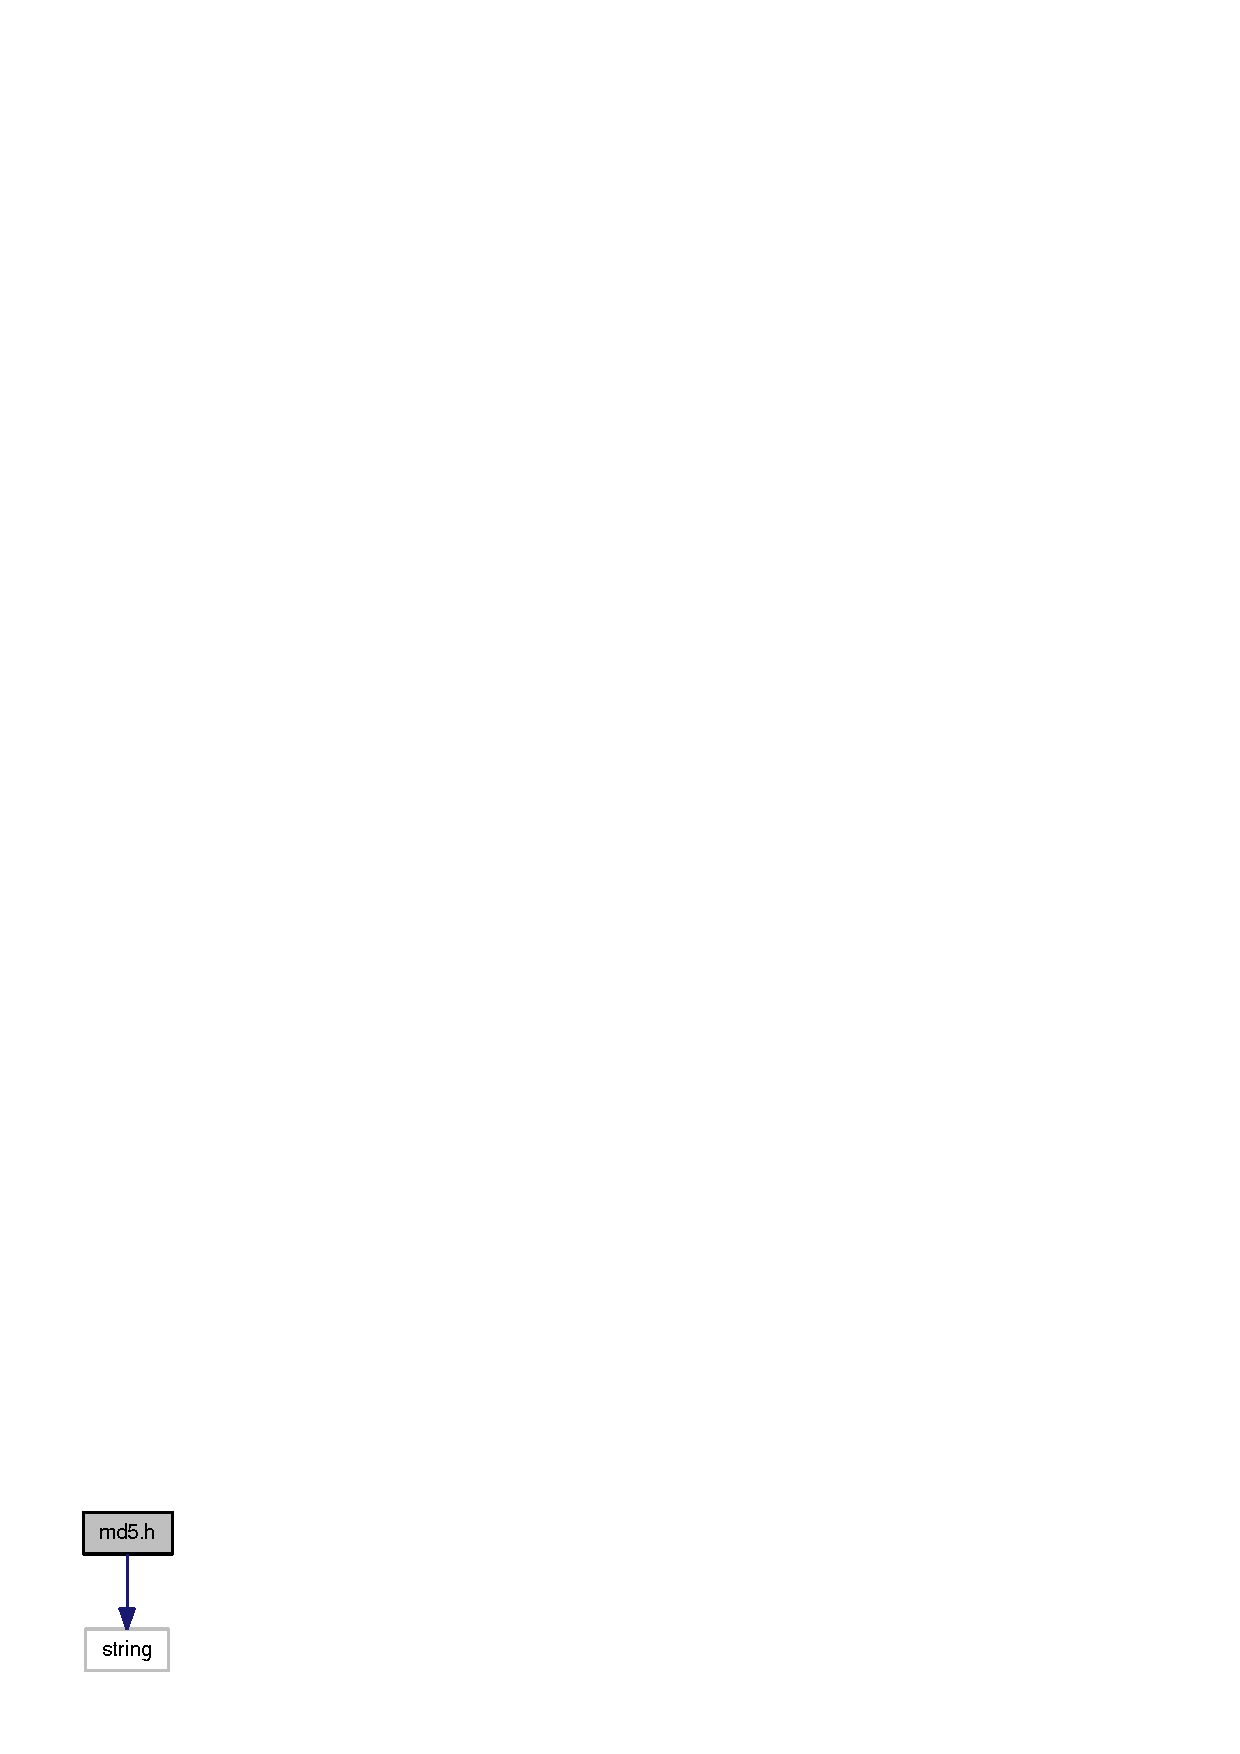
\includegraphics[width=234pt]{d5/db6/a00042}
\end{center}
\end{figure}

\printindex
\end{document}
